\documentclass[journal]{IEEEtran}
\IEEEoverridecommandlockouts
% SCooP-iT, IEEE Internet of Things Journal (IoT-J) submission draft.
% Built from ../scoop_testbed_paper (the RA-L draft). Framing: the robots
% and masts are mobile and fixed IoT nodes on one contended Wi-Fi network,
% and cooperative perception is the application whose outcome the network
% decides.
%
% Length: compiled 15 pages including 2.5 pages of references (18 before
% the cuts of DIRECTION.md, Sec. 3). Check the current IoT-J length policy
% in the Author Portal; the rest is closed by condensing prose.
% Supplementary material: supplementary.tex (compile separately).
% Companion: the SCooP dataset paper (cited as scoop_dataset).

\usepackage{cite}
\usepackage{amsmath,amssymb,amsfonts}
\usepackage{algorithmic}
\usepackage{graphicx}
\usepackage{textcomp}
\usepackage{xcolor}
\usepackage{tabularx}
\usepackage{multirow}
\usepackage{array}
\usepackage{booktabs}
\usepackage{siunitx}
\usepackage[hidelinks]{hyperref}

\graphicspath{{figures/}}

\definecolor{darkyellow}{RGB}{180,140,0}
\definecolor{darkgreen}{RGB}{0,150,20}

% Red TODO markers -- search for \todo before submission; none may remain.
\newcommand{\todo}[1]{\textcolor{red}{[TODO: #1]}}
\newcommand{\unsure}[1]{\textcolor{darkyellow}{[UNSURE: #1]}}
\newcommand{\bib}[1]{\textcolor{darkgreen}{[BIB: #1]}}
\newcommand{\Ttransform}[2]{\ensuremath{T_{\mathrm{#1}}^{\mathrm{#2}}}}
\newcommand{\cmark}{$\checkmark$}
\newcommand{\xmark}{--}

\renewcommand{\floatpagefraction}{0.8}

\begin{document}

\title{SCooP-iT: A Real-World Indoor Testbed and Environment for
Embodied Multi-Agent Perception}

\author{Jorich Loquero and Ming-Chun Lee,~\IEEEmembership{Member,~IEEE}%
\thanks{Manuscript received Month DD, YYYY; revised Month DD, YYYY;
accepted Month DD, YYYY. \todo{Funding.}}%
\thanks{The authors are with the Department of Electrical and Computer
Engineering, National Yang Ming Chiao Tung University, Hsinchu, Taiwan
(e-mail: jorich.ee14@nycu.edu.tw; \todo{email}).}%
\thanks{Digital Object Identifier (DOI): see top of this page.}}

\markboth{IEEE Internet of Things Journal,~Vol.~XX, No.~XX, Month~YYYY}%
{Loquero \MakeLowercase{\textit{et al.}}: SCooP-iT: A Real-World Indoor Testbed and Environment for Embodied Multi-Agent Perception}

\maketitle

% Abstract and index terms.
% Writing order: real-world problem -> what SCooP-iT captures -> how it is
% validated -> what others can do with it (replay, Gym) -> results.
\begin{abstract}
Methods for teams of robots and fixed sensors that share what they
perceive are developed on vehicle datasets and in simulation, yet a
real indoor team differs on every layer at once: its sensors fall short
and differ between agents, it has no GNSS to tell where an agent was,
and its agents share one contended wireless network. We present
SCooP-iT, a real-world indoor testbed and environment in which a
heterogeneous team, a LiDAR robot, an RGB-D cart, and camera--radar
infrastructure masts, is captured on one clock and in one metric frame
without motion capture or GNSS. Sensing and communication are recorded
together: every inter-agent link is logged on the sensors' clock as
link state at \SI{5}{\hertz}, round-trip time at \SI{100}{\hertz},
goodput in \SI{4}{\second} windows, and Wi-Fi channel state at
\SIrange{104}{141}{\hertz}; clocks agree to below
\SI{1}{\milli\second}; and a self-built reference map with a fiducial
chain places every agent to \SI{10}{\milli\metre} (LiDAR robot) and
\SIrange{31}{54}{\milli\metre} (RGB-D cart) on held-out fiducials. The
capture is offered for use in three ways: the recordings as a test
bench into which any collaborative method is replayed against the link
the agents actually had; SCooP-iT Gym, a closed-loop multi-agent
environment with a Gymnasium interface whose world, sensors, link, and
failure conditions are built from the recordings; and the testbed
itself, on which a policy trained in the Gym is deployed and checked.
Experiments show that the testbed's own errors are 6--101$\times$
smaller than the effects it measures; that its map predicts the radio
signal it logs although neither produced the other (Spearman
$\rho = 0.60$, \SI{5.4}{\decibel} clear-to-obstructed drop);
\todo{that replay reproduces live arrivals and the Gym's world
reproduces the real scans, link, and task}; and that the real world
hides what simulation shows as solved: under contention, a link whose
round trip of \SIrange{25}{33}{\milli\second} sits well inside one
\SI{100}{\milli\second} LiDAR frame still delivers only
\SIrange{59}{68}{\percent} of \SI{1.5}{\mega\byte} messages within it,
against 100\,\% under the synthetic channels of prior benchmarks.
SCooP-iT is the acquisition platform of the SCooP dataset.
\end{abstract}

\begin{IEEEkeywords}
Internet of Robotic Things, testbed, embodied multi-agent perception,
cooperative perception, digital twin, multi-agent environment, Wi-Fi,
channel state information, time synchronization, ground truth
\end{IEEEkeywords}


%=======================================================================
% Sec. I Introduction (about 1 page).
% Paragraphs: (1) the real-world gap; (2) IoRT and the surveys: why now;
% (3) why indoors is hard on every layer; (4) no existing platform;
% (5) SCooP-iT and its three uses; (6) contributions; (7) seven questions
% and the roadmap.
\section{Introduction}
\label{sec:introduction}
\IEEEPARstart{T}{eams} of robots and fixed sensors that share what they
perceive can see beyond the occlusions of any one of them. They
cooperate through collaborative SLAM, which places every agent in one
shared map \cite{swarmslam,doorslam,kimeramulti}, and cooperative
perception, which fuses what the agents observe within it
\cite{where2comm,zhou2022gnnperception}. The methods for both are
developed on vehicle datasets and in simulation
\cite{opv2v,v2xsim,dairv2x,v2v4real}, where agents carry the same
sensors, ground truth comes from GNSS, and messages arrive on time. A
real indoor team differs on every layer at once. Its sensors fall
short of their nominal rates and differ from agent to agent; its
clocks drift; there is no GNSS to tell where an agent was; the
building occludes cameras and radio alike; and its agents share one
contended wireless network, so a neighbor's message may arrive after
the scene has changed. Data freshness, studied as the age of
information \cite{kaul2012aoi,yates2021aoi}, here has a concrete
deadline of one sensor frame.

The Internet of Robotic Things treats such robots as mobile nodes that
sense and share data over the same network as fixed devices
\cite{simoens2018iort}. Recent surveys of networked embodied
intelligence draw the consequence for evaluation: delivering a message
is only an intermediate step whose value depends on whether it arrives
in time for the task, so sensing, communication, and the task outcome
have to be measured together \cite{zhang2026mean}. They and surveys of
embodied multi-robot systems name the missing instrument: benchmarks
evaluate communication, robotics, or perception separately, most in
simulations that overlook real sensing and communication, and
integrated testbeds with real wireless dynamics, heterogeneous agents,
and multi-agent tasks, bridged to simulation, are an open problem
\cite{zhang2026mean,wen2026embodiedmrs}.

Building such an instrument indoors is hard on every layer. Each
agent's sensing must be on one timeline with every other's, with a
bound on the error; each agent must have a pose in one metric frame
at building scale, without motion capture or GNSS; each link must be
recorded per agent pair, with the channel beneath it; and, for the
instrument to be used by others, the capture must be replayable into a
new method and extensible into situations it did not record.

No existing platform provides this. IoT and wireless testbeds measure
the radio but run no scored task
\cite{adjih2015iotlab,breen2021powder,raychaudhuri2020cosmos,bonati2021colosseum}.
Wi-Fi channel datasets measure CSI on dedicated sounding links, with
positions from a survey instrument \cite{dichasus,espargos}.
Communication-aware robot systems run over real links that they
monitor but do not release, and score nothing against a reference
\cite{ginting2021chord,saboia2022achord,cladera2024mocha}.
Cooperative-perception platforms are outdoor and GNSS-referenced, and
reduce the measured link to a scalar delay or a live run
\cite{v2v4real,zimmer2024tumtrafv2x,v2xrealo,cooperscene}. Embodied
multi-agent environments are simulated, with generated worlds and an
ideal network \cite{lingjing}.

This paper presents SCooP-iT, the indoor testbed of SCooP (Sensing and
Communication for Cooperative Perception): a real-world testbed in
which a heterogeneous team is captured on one clock and in one frame,
sensing and communication alike, and an environment built from that
capture. It is meant to be used in three ways. The \emph{recordings}
are a test bench: any collaborative method is replayed on what the
agents sensed and against the link they had. \emph{SCooP-iT Gym} is a
closed-loop environment whose world, sensors, link, and failure
conditions are built from the recordings, in which agents are trained
where the recordings cannot go. And the \emph{testbed} itself closes
the loop: a policy trained in the Gym is deployed on the real agents,
and what happened is compared with what the Gym predicted. Each use is
validated against reality. The contributions are:
\begin{enumerate}
    \item \textbf{A heterogeneous indoor testbed with sensing and
    communication on one clock}: two mobile and three infrastructure
    agents on one access point, every pair's link recorded (passive
    state at \SI{5}{\hertz}, RTT at \SI{100}{\hertz}, goodput in
    \SI{4}{\second} windows, CSI at \SIrange{104}{141}{\hertz}),
    contention as a controlled knob, and measured clock offsets below
    \SI{1}{\milli\second} (Secs.~\ref{sec:design}, \ref{sec:alignment},
    \ref{sec:link}).
    \item \textbf{Building-scale ground truth without motion capture,
    GNSS, or surveyed anchors}: a self-built reference map and a
    fiducial chain for agents without LiDAR, validated by measurements
    that never enter it, \todo{cross-pass figure} and
    \SI{10}{\milli\metre} against held-out fiducials
    (Sec.~\ref{sec:gt}).
    \item \textbf{A replay validated against live runs}: the recorded
    per-pair, per-message link, and the other recorded conditions, fed
    into any collaborative method keyed to sensor time,
    \todo{validated against live execution to within one receiver
    frame} (Sec.~\ref{sec:replay}, E3).
    \item \textbf{SCooP-iT Gym}: a closed-loop multi-agent environment
    with a Gymnasium interface, whose building, sensors, motion, link,
    and failure conditions are built from the recordings and each
    checked against held-out real runs, with every failure traced to
    its cause, and a train--test--deploy protocol that ends on the real
    testbed (Sec.~\ref{sec:gym}).
    \item \textbf{What the real world shows that simulation hides}: with
    a second robot on the access point, the loaded round trip of
    \SIrange{25}{33}{\milli\second} stays well inside one
    \SI{100}{\milli\second} LiDAR frame, yet only
    \SIrange{59}{68}{\percent} of \SI{1.5}{\mega\byte} messages arrive
    within it (86\,\% with one robot), while the synthetic channels of
    prior benchmarks deliver 100\,\% (Sec.~\ref{sec:experiments}).
\end{enumerate}

A testbed paper is judged on seven questions, five about whether the
instrument can be trusted and two about whether it is worth having
(Table~\ref{tab:spec}): \emph{Is it precise?} Are its own errors small
next to the effects it measures (E1)? \emph{Is it consistent?} Do the
poses and the link logs agree when neither was checked by hand (E2)?
\emph{Is it faithful?} Do the replay and the Gym reproduce what the
real agents sensed, sent, and achieved (E3)? \emph{Is it repeatable?}
Does the same setting give the same link on another day (E4)? \emph{Is
it necessary?} What does the real world show that a synthetic one
hides (E5)? \emph{Is it unique?} What can it do that no existing
platform can (Sec.~\ref{sec:related})? \emph{Is it reproducible?} Can
someone else build and use it (Secs.~\ref{sec:design},
\ref{sec:lessons})? Each trust question has a pass criterion fixed
before the data were read. Sec.~\ref{sec:related} reviews related work;
Secs.~\ref{sec:design}--\ref{sec:replay} describe the testbed and its
replay; Sec.~\ref{sec:experiments} reports the experiments;
Sec.~\ref{sec:gym} presents the Gym and its train--test--deploy
protocol; and Sec.~\ref{sec:lessons} gives the lessons the real world
taught and the limitations. The sequences and labels recorded on the
testbed are released as the SCooP dataset \cite{scoop_dataset}.


%=======================================================================
% Sec. Related Work
\section{Related Work}
\label{sec:related}

A team of robots and fixed sensors that shares perception over Wi-Fi
is an IoT system: heterogeneous nodes sense, compute, and exchange
data over one shared, contended network, and the application succeeds
only if each message arrives while it is still fresh
\cite{simoens2018iort}. Surveys of networked embodied intelligence
organize its evaluation in levels, communication and computation
indicators below and embodied task indicators above, and argue that
only their joint measurement shows whether a network serves a task
\cite{zhang2026mean}; surveys of embodied multi-robot systems find that
benchmarks overlook communication latency and call for frameworks that
evaluate perception and communication across heterogeneous teams, with
hardware in the loop \cite{wen2026embodiedmrs}. Studying such a system
needs four things at
once: the network measured where the application runs, the channel
beneath it, every node's position and clock, and a way to put a new
application on the same network again. We review IoT testbeds, network
timeliness, wireless channel measurement, robots as IoT nodes, and
cooperative perception as the application, and close with the gap at
their intersection.

\subsection{IoT and Wireless Experimentation Testbeds}
Open testbeds made IoT and wireless experiments reproducible at scale.
FIT IoT-LAB \cite{adjih2015iotlab} reported 2,728 low-power nodes and
117 mobile robots across six indoor sites; its robots log their own
pose estimate, and its nodes record received power per channel. The
PAWR platforms POWDER \cite{breen2021powder} and COSMOS
\cite{raychaudhuri2020cosmos} provide city-scale software-defined
radio and edge computing, with small indoor labs beside the outdoor
deployment, and Colosseum \cite{bonati2021colosseum} emulates the RF
channel in FPGA hardware between 128 radios from modeled, ray-traced,
or measured scenarios. These testbeds make the radio the object of
study. Link metrics are instrumented by the experimenter, node
positions come from GNSS or the node itself, and no application task
is scored against ground truth, so they show what the network did but
not what it did to an application.

\subsection{Timeliness and Networking for IoT Applications}
The throughput of a contended 802.11 cell is modeled analytically
\cite{bianchi2000dcf}, and the freshness of status updates is captured
by the age of information \cite{kaul2012aoi,yates2021aoi}.
Task-oriented communication encodes features for a downstream
inference task rather than for reconstruction
\cite{shao2022taskoriented}, and edge computing for connected vehicles
\cite{liu2019edgeav} and cloud robotics \cite{kehoe2015cloud} place
the network on the critical path of perception. For robots, ROS~2
middleware (DDS, Zenoh, MQTT) has been benchmarked over Ethernet,
Wi-Fi, and 4G \cite{zhang2024ros2middleware}. Clocks are aligned by
NTP \cite{mills1991ntp} or, in sensor networks, by FTSP
\cite{maroti2004ftsp}. Measured networks are replayed by trace-driven
emulators \cite{noble1997trace,winstein2013sprout,netravali2015mahimahi,yan2018pantheon,hemminger2005netem}.
These works analyze, encode for, or emulate the network under
saturated, synthetic, or recorded traffic, but the deadline they
evaluate against is not that of a sensing application on the same
nodes, and a replayed trace feeds a socket, not a multi-node
application keyed to sensor time.

\subsection{Wireless Channel Measurement and Prediction}
Commodity CSI extraction, first on the Intel~5300
\cite{halperin2011csitool}, then with Nexmon \cite{nexmon} and
PicoScenes \cite{jiang2022picoscenes}, turned Wi-Fi into a sensor
\cite{ma2019wifisensing}. Channel datasets pair CSI or beam power with
positions or other modalities: DICHASUS \cite{dichasus} sounds a
distributed massive-MIMO channel indoors and outdoors with tachymeter
and GNSS positions, ESPARGOS \cite{espargos} records phase-coherent
Wi-Fi CSI from a robot-borne transmitter tracked by a total station,
MM-Fi \cite{mmfi} pairs CSI with human pose, and DeepSense~6G
\cite{deepsense6g} pairs mmWave beam power with camera, LiDAR, radar,
and RTK positions. Ray-traced digital twins
\cite{hoydis2023sionnart,alkhateeb2023digitaltwin,bostontwin,deepmimo}
and learned radio maps \cite{levie2021radiounet} predict the channel
from geometry. In this line, CSI is measured on dedicated sounding
links or used to sense people and passive targets, rather than on the
links over which IoT nodes exchange their application data; positions
come from a survey instrument or GNSS; and geometry is an input to
channel prediction, not an independent reference against which the
measured channel is checked.

\subsection{Robots as Mobile IoT Nodes}
The Internet of Robotic Things treats robots as mobile nodes that
sense, act, and share data over the same network as other devices
\cite{simoens2018iort}. Communication-aware robotics plans motion
around the channel \cite{muralidharan2021commaware}: robots map signal
strength online \cite{fink2010radiomap} or exploit its directionality
to keep a team connected \cite{gil2015adaptive}. CHORD and ACHORD
\cite{ginting2021chord,saboia2022achord} share data over intermittent
links in subterranean deployments of the DARPA SubT Challenge,
monitoring per-link SNR to route over dropped relays, and MOCHA
\cite{cladera2024mocha} does so in outdoor air--ground field trials,
synchronizing when the received signal strength allows. ROS-NetSim
\cite{calvofullana2021rosnetsim} routes real ROS traffic through a
simulated network. Multi-robot testbeds such as the Robotarium
\cite{wilson2021robotarium}, the CPM Lab \cite{kloock2021cpmlab}, and
ChoiRbot \cite{testa2021choirbot} obtain positions from overhead
cameras or motion capture and treat the network as ideal. Indoors
without motion capture, a pose reference needs surveyed UWB anchors
\cite{zhao2024util}, total-station points \cite{hilti2022}, surveyed
fiducials \cite{airmuseum}, or a scanner-built prior map
\cite{subtmrs,lamar}; SLAM-derived references are validated by sparse
landmark distances \cite{incrowdvi} or by internal consistency alone
\cite{envodat}. Robots therefore run over real links that are
monitored but not released, or have precise positions over a network
assumed ideal; none has both on one timeline, and none scores an
application against an independent reference.

\subsection{Cooperative Perception as an IoT Application}
Cooperative perception fuses raw points \cite{chen2019cooper},
features \cite{chen2019fcooper,wang2020v2vnet}, or selected regions
\cite{where2comm,liu2020when2com} from several nodes; F-Cooper
\cite{chen2019fcooper} frames it as an edge-computing system. Methods
now target what the network does to the fused result: latency
\cite{lei2022syncnet,v2xvit}, asynchrony \cite{wei2023cobevflow},
interruptions and packet loss \cite{ren2024v2xincop}, and pose error
\cite{lu2023coalign}. They are trained on simulated or outdoor data
\cite{opv2v,v2xsim,dairv2x} and evaluated against a constant delay, a
Bernoulli drop, or no latency, with pose error drawn from a chosen
distribution. Real-world platforms are outdoor and vehicular. V2V4Real
\cite{v2v4real} and TUMTraf-V2X \cite{zimmer2024tumtrafv2x} provide
GNSS-referenced multi-agent data with synchronization of tens of
milliseconds and no link log; \cite{hawlader2024v2xexp} reports V2X
experiments on real hardware; V2X-ReaLO \cite{v2xrealo} runs online
fusion over a live Wi-Fi link and reports its latency; and CooperScene
\cite{cooperscene}, the nearest case, releases pairwise C-V2X latency,
throughput, loss, and jitter traces with PTP-synchronized sensors, and
evaluates detectors under a delay derived from the measured mean
throughput. CoPeD \cite{coped}, an air--ground team recorded indoors
and outdoors, takes pose from its own visual-inertial odometry fused
with GPS and logs no link. The link, where recorded, is measured at or
above the transport layer without channel state, and it enters the
evaluation as a scalar delay or a live run, not as the per-message
trace each node actually had.

\subsection{Simulators and Environments for Embodied Agents}
Embodied agents are trained in simulators that generate their world:
Habitat \cite{habitat} for indoor navigation, CARLA \cite{carla} and
OpenCDA \cite{xu2021opencda} for driving, the latter generating the
cooperative-perception data of OPV2V \cite{opv2v}, and Isaac Lab
\cite{orbit} on Isaac Sim \cite{isaacsim} for robot learning at GPU
scale, behind the Gymnasium and PettingZoo interfaces
\cite{gymnasium,pettingzoo}. Lingjing \cite{lingjing} runs heterogeneous
aerial and ground agents in a simulated city behind a Gym-like
interface, with star or broadcast communication and episodes replayed
for failure attribution, but its messages pass an ideal bus whose cost
is a message count, never a delay or a loss. Driving research grounds
closed-loop simulation in real logs instead: nuPlan \cite{nuplan} and
Waymax \cite{waymax} replay recorded scenes around a simulated ego.
These environments either generate the world or replay it for one ego
over no network; none builds a multi-agent environment from a real
team's sensing and communication and checks it against that team.

\subsection{The Gap at the Intersection}
Table~\ref{tab:gap_iotj} compares the closest platforms on link,
channel, clock, pose reference, and replay; the supplementary material
states each gap by discipline, what SCooP-iT provides, and where the
paper shows it. IoT testbeds measure
the network but run no scored application; channel datasets measure
CSI on sounding links under a survey instrument; robot systems run
over real links but release no link log and score nothing; and
cooperative-perception platforms score the application outdoors under
GNSS but reduce the link to a scalar delay or a live run; and embodied
environments generate their world over an ideal network. SCooP-iT is
an indoor IoT testbed in which heterogeneous mobile and fixed nodes
record per-pair link and channel state on the sensors' clock, with a
measured bound on that clock, have a validated pose for every scan
without motion capture or GNSS, and replay the recorded per-message
link into any collaborative application, and build a closed-loop
environment from the same capture that is checked against it. It is the
integrated testbed the surveys call for
\cite{zhang2026mean,wen2026embodiedmrs}: sensing, communication, and
the task outcome of every run on one timeline, bridged to simulation by
an environment that answers to the real runs.

% Table II: related platforms, every cell checked on 18 Oct 2026 against
% official repos, project documentation, and excerpts of the papers
% (ACHORD paper, MOCHA and CPM Lab code read in full). Re-check against
% the PDFs before submission; arXiv and IEEE Xplore were not reachable.
\begin{table*}[!t]
\caption{Related IoT Testbeds, Channel Datasets, Networked Robots, and
Cooperative-Perception Platforms Compared on Link, Channel, Clock, Pose
Reference, and Replay}
\label{tab:gap_iotj}
\begin{center}
\renewcommand{\arraystretch}{1.15}
\setlength{\tabcolsep}{2pt}
\scriptsize
\begin{tabularx}{\textwidth}{@{}l l >{\raggedright\arraybackslash}p{1.3cm} c >{\raggedright\arraybackslash}X >{\raggedright\arraybackslash}p{1.1cm} >{\raggedright\arraybackslash}p{1.3cm} >{\raggedright\arraybackslash}p{1.4cm} >{\raggedright\arraybackslash}p{1.1cm} >{\raggedright\arraybackslash}p{1.1cm}@{}}
\toprule
\textbf{Platform} & \textbf{Venue} & \shortstack[l]{\textbf{Nodes}\\\textbf{(mob./fixed)}} & \textbf{Indoor} & \textbf{Measured link} & \textbf{CSI} & \shortstack[l]{\textbf{Pose}\\\textbf{reference}} & \shortstack[l]{\textbf{Clock}\\\textbf{sync}} & \shortstack[l]{\textbf{Link}\\\textbf{replay}} & \shortstack[l]{\textbf{App.}\\\textbf{scoring}} \\
\midrule
\multicolumn{10}{@{}l}{\textit{IoT and wireless testbeds}} \\
FIT IoT-LAB \cite{adjih2015iotlab} & WF-IoT'15 & 117 / 2728 & \cmark & Partial: RSSI per channel at node & \xmark & Self-estimate & Partial: GPS, subset & \xmark & \xmark \\
POWDER \cite{breen2021powder} & ComNet'21 & 20 / sites & partial & Partial: user-instrumented & Raw IQ & GNSS & Partial: GPSDO & \xmark & \xmark \\
COSMOS \cite{raychaudhuri2020cosmos} & MobiCom'20 & $\sim$200 / $\sim$50$^a$ & partial & Partial: user-instrumented & Raw IQ & Not reported & Not reported & \xmark & \xmark \\
Colosseum \cite{bonati2021colosseum} & DySPAN'21 & 128 emul. & --- & Emulated per pair & Emul.\ CIR & --- & Not reported & RF replay & \xmark \\
\midrule
\multicolumn{10}{@{}l}{\textit{Wi-Fi CSI tools and channel datasets}} \\
Nexmon CSI \cite{nexmon} & WiNTECH'19 & tool & --- & Partial: per-frame RSSI & \cmark & --- & \xmark & \xmark & \xmark \\
PicoScenes \cite{jiang2022picoscenes} & IoT-J'22 & tool & --- & Partial: per-frame RSSI, SNR & \cmark & --- & \xmark & \xmark & \xmark \\
DICHASUS \cite{dichasus} & WSA'21 & 1 / arrays & partial & --- & Sounding link & Tachymeter, DGNSS & Partial: OTA ref. & \xmark & \xmark \\
ESPARGOS \cite{espargos} & arXiv'24 & 1 / 4 arrays & \cmark & --- & Receive-only & Total station & Partial: shared clock & \xmark & \xmark \\
DeepSense 6G \cite{deepsense6g} & ComMag'23 & 1 / 1 & partial & Partial: beam power & \xmark & RTK & Partial: UTC stamps & \xmark & \xmark \\
\midrule
\multicolumn{10}{@{}l}{\textit{Robots as IoT nodes}} \\
Robotarium \cite{wilson2021robotarium} & RA-L'21 & $N$ / 0 & \cmark & --- & \xmark & Overhead tracking & \xmark & \xmark & \xmark \\
CPM Lab \cite{kloock2021cpmlab} & ECC'21 & $N$ / 0 & \cmark & Aggregate RTT (UI only) & \xmark & Overhead camera & NTP, no bound & \xmark & \xmark \\
ChoiRbot \cite{testa2021choirbot} & RA-L'21 & $N$ / 0 & \cmark & --- & \xmark & Motion capture & \xmark & \xmark & \xmark \\
CHORD / ACHORD \cite{ginting2021chord,saboia2022achord} & RA-L'21/'22 & 6 / base + relays & subterr. & Partial: per-link SNR, not released & \xmark & \xmark & \xmark & \xmark & \xmark \\
MOCHA \cite{cladera2024mocha} & ICRA'24 & UAV+UGVs / base & \xmark & Partial: per-peer RSSI, RTT, bandwidth, not released & \xmark & Not reported & \xmark & \xmark & \xmark \\
ROS-NetSim \cite{calvofullana2021rosnetsim} & RA-L'21 & sim. & --- & Simulated & \xmark & --- & \xmark & Sim. & \xmark \\
Mahimahi / NetEm \cite{netravali2015mahimahi,hemminger2005netem} & ATC'15 / LCA'05 & --- & --- & Recorded trace & \xmark & --- & \xmark & Transport & \xmark \\
\midrule
\multicolumn{10}{@{}l}{\textit{Cooperative-perception platforms}} \\
CoPeD \cite{coped} & RA-L'24 & 5 / 0 & partial & --- & \xmark & VIO + GPS & NTP, no number & \xmark & Partial$^b$ \\
V2V4Real \cite{v2v4real} & CVPR'23 & 2 / 0 & \xmark & --- & \xmark & GNSS/INS & Partial: $<$\,50\,ms & \xmark & Det., track. \\
TUMTraf-V2X \cite{zimmer2024tumtrafv2x} & CVPR'24 & 1 / 1 & \xmark & --- & \xmark & RTK & Partial: 24.9\,ms & \xmark & Det., track. \\
V2X-ReaLO \cite{v2xrealo} & arXiv'25 & 2 / 2 & \xmark & Latency (Wi-Fi) & \xmark & GNSS & No number & Live only & Det.\ (online) \\
CooperScene \cite{cooperscene} & ECCV'26 & 3 / 1 & \xmark & Pairwise C-V2X RTT, throughput, loss, jitter & \xmark & RTK + ICP & Claimed sub-ms & Scalar delay$^c$ & Detection \\
AutoCast \cite{qiu2022autocast} & MobiSys'22 & sim. & \xmark & Simulated & \xmark & Simulator & \xmark & Sim. & Sim. \\
\midrule
\textbf{SCooP-iT (ours)} & --- & 2 / 3 & \cmark & RSSI, MCS, retries (5\,Hz), RTT (100\,Hz), goodput (4\,s), per pair & \cmark$^d$ & Map + fiducials & Measured & Per message & C-SLAM, det. \\
\bottomrule
\end{tabularx}
\end{center}
\vspace{2pt}
{\scriptsize \cmark: provided; partial: provided in part, or only if the experimenter instruments it; \xmark: not provided; ---: not applicable.\quad
$^a$Planned deployment in the 2020 paper.\quad
$^b$Zero-shot foundation-model image labels, no 3D boxes.\quad
$^c$One delay derived from mean measured throughput, not a per-message trace.\quad
$^d$Single-antenna Wi-Fi CSI on the data links (BCM43455c0, \SI{80}{\mega\hertz}, \SIrange{104}{141}{\hertz}), not phase-coherent across nodes.}
\end{table*}



%=======================================================================
% Sec. Testbed Design
\section{Testbed Design}
\label{sec:design}
SCooP-iT consists of two mobile agents and three infrastructure
agents connected to a single access point, with an additional host
that extracts channel state. In IoT terms each agent is a node that
senses, computes, and communicates: the mobile agents are mobile IoT
nodes, the masts fixed ones, and the access point the shared network
whose behavior the testbed measures. Fig.~\ref{fig:overview} shows a recording
scenario with the agents placed in the map frame and the measured
links between them. \todo{Redraw Fig.~\ref{fig:overview} per the plan:
floor plan with agents in the map frame, links colored by measured RTT
or RSSI, and a strip below with one shared timeline of sensor frames,
link samples, and CSI. It should say ``one clock, one frame, every
link'' without text.}

\begin{figure}[t]
\centering
\fbox{\parbox[c][5cm][c]{0.95\columnwidth}{\centering
\todo{Fig.~1: one window of \texttt{coop\_2} on one timeline. Top: floor
plan with both robots' paths and the masts in the map frame, the
robot-to-AP paths coloured by Fresnel clearance. Below, stacked on a
shared time axis: clearance, RSSI, RTT, goodput, and each
\SI{1.5}{\mega\byte} message's predicted arrival against the
\SI{100}{\milli\second} frame boundary.}}}
\caption{SCooP-iT in one window: agents in one map frame, every link
measured, one clock. Where the map shows the path obstructed, the
signal drops, goodput falls, and large messages miss their frame.}
\label{fig:overview}
\end{figure}


\subsection{Agents}
\texttt{mobile\_1}, the LiDAR robot, is an AgileX Scout Mini equipped
with an Ouster OS1-64 LiDAR, a ZED~2i stereo camera with an integrated IMU,
two IWR6843 mmWave radars, and an RTL8852BU Wi-Fi interface. It also
carries \texttt{sniffer}, a Raspberry Pi~4 whose BCM43455c0 chipset is
used for CSI extraction. \texttt{mobile\_2}, the RGB-D cart, is a
pushcart equipped with an Ouster OS1-128 LiDAR, a RealSense D455 RGB-D
camera with IMU, an on-board visual SLAM pipeline, and a Wi-Fi interface \todo{Add Radar
(?)}. Each infrastructure mast, \texttt{infra\_N}, carries an Arducam
RGB camera, an IWR6843 radar, and a Raspberry Pi whose on-board
BCM43455 serves as the wireless interface. The sensor models, rates,
and resolutions are listed in Table~\ref{tab:sensors}; compute,
storage, and cost per agent class are given in Table~\ref{tab:bom}.
The three classes are deliberate: the LiDAR robot builds the reference
map, the cart represents the low-cost agents a deployed team contains
and that a reference must localize without a LiDAR, and the masts
provide the elevated, persistent vantage no mobile node can sustain.

\begin{figure*}[t]
\centering
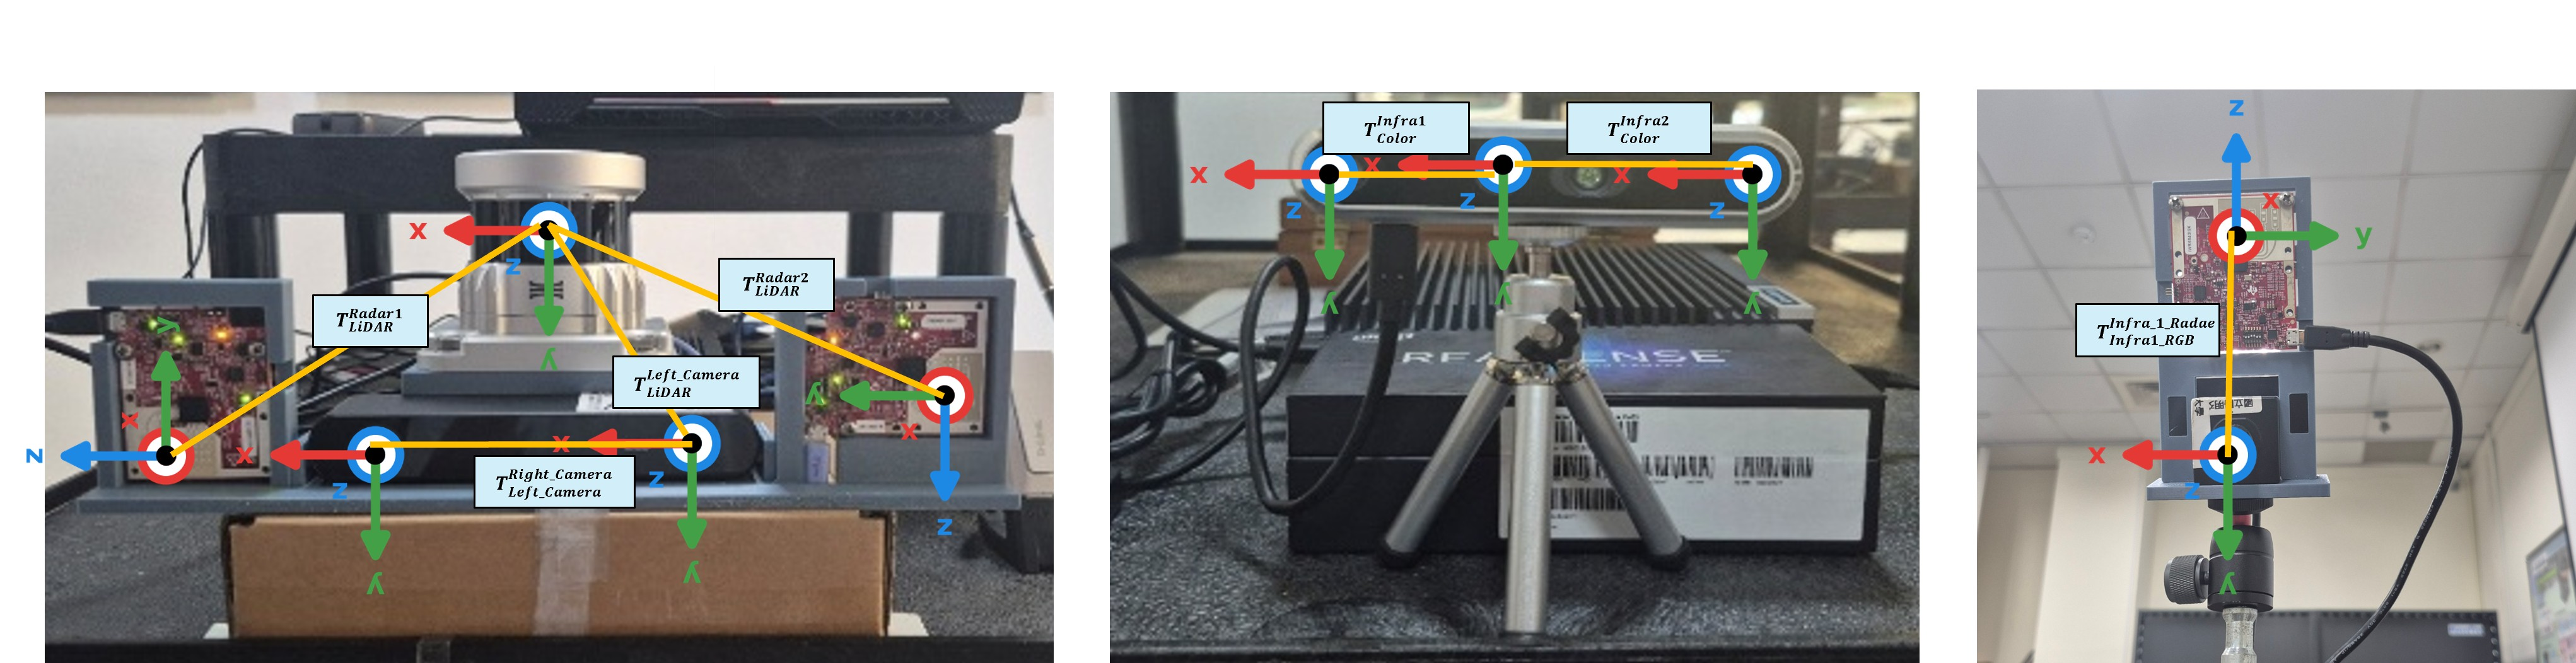
\includegraphics[width=\textwidth]{figs/fig02_platforms.jpg}
\caption{Platforms and frames. Axes mark each sensor frame (x red,
y green, z blue); yellow arrows are the extrinsic transforms
estimated in Sec.~\ref{sec:alignment}. \texttt{mobile\_1} uses
\texttt{base\_link} as origin (not shown here), \texttt{mobile\_2} its LiDAR, and the
infrastructure rig its camera.}
\label{fig:platforms}
\end{figure*}

\begin{table}[t]
\centering
\caption{Sensing per agent class (full specification in the
supplementary material).}
\label{tab:sensors}
\footnotesize
\setlength{\tabcolsep}{3pt}
\begin{tabularx}{\columnwidth}{@{}l>{\raggedright\arraybackslash}Xl@{}}
\toprule
Agent & Sensor & Rate \\
\midrule
\multirow{5}{*}{\texttt{mobile\_1}} & Ouster OS1-128 / OS0-64 LiDAR & \SI{10}{\hertz} \\
 & ZED 2i stereo (1920$\times$1080) + IMU & 30 / \SI{400}{\hertz} \\
 & 2$\times$ TI IWR6843ISK \SI{60}{\giga\hertz} radar & \SI{10}{\hertz} \\
 & RTL8852BU 802.11ac Wi-Fi & 5 / \SI{100}{\hertz} \\
 & \texttt{sniffer}: RPi 4B BCM43455c0 CSI (242 sc.) & $\sim$\SIrange{100}{140}{\hertz} \\
\midrule
\multirow{3}{*}{\texttt{mobile\_2}} & RealSense D455 RGB-D (1280$\times$800) & \SI{30}{\hertz} \\
 & IMU BMI055; on-board visual SLAM & 200 / \SI{30}{\hertz} \\
 & 802.11ac Wi-Fi & 5 / \SI{100}{\hertz} \\
\midrule
\multirow{3}{*}{\texttt{infra\_N}} & Arducam B0495 RGB (1920$\times$1200) & \SI{30}{\hertz} \\
 & TI IWR6843ISK radar & \SI{10}{\hertz} \\
 & RPi 4B BCM43455 Wi-Fi & 5 / \SI{100}{\hertz} \\
\bottomrule
\end{tabularx}
\end{table}


\begin{table}[t]
\centering
\caption{Bill of materials and per-site setup effort. \todo{Fill costs and effort.}}
\label{tab:bom}
\footnotesize
\setlength{\tabcolsep}{4pt}
\begin{tabularx}{\columnwidth}{@{}l>{\raggedright\arraybackslash}Xr@{}}
\toprule
Agent class & Main components & Cost \\
\midrule
LiDAR robot (\texttt{mobile\_1}) & Scout Mini, Ouster OS1-64, ZED 2i, 2$\times$ IWR6843ISK, Jetson AGX Orin, RTL8852BU, RPi 4B sniffer & \todo{} \\
RGB-D cart (\texttt{mobile\_2}) & Pushcart, Ouster OS1-128, RealSense D455, compute \todo{}, Wi-Fi & \todo{} \\
Infrastructure mast (\texttt{infra\_N}) & Mast, Arducam B0495, IWR6843ISK, RPi 4B & \todo{} \\
Network & 1 access point (802.11ac, VHT-80), rangefinder, printed ChArUco boards & \todo{} \\
\midrule
\multicolumn{3}{@{}l}{\emph{Per new site:} mapping session \todo{min}; \todo{N} boards; \todo{N} rangefinder distances; second pass optional} \\
\bottomrule
\end{tabularx}
\end{table}


\subsection{Network}
All agents associate to a single access point on channel 149 (VHT-80,
\SI{5745}{\mega\hertz}); no ad hoc or mesh mode is used, and power
save is disabled on all transmitters. The transmitter settings are
imposed by the CSI receiver: a 1$\times$1 802.11ac configuration.
802.11ax is disabled, since the receiver cannot demodulate HE frames
and would capture only control frames, and the number of spatial
streams is fixed to one, since a single-antenna receiver cannot
separate a two-stream transmission. The measured single-stream
capacity is \numrange{275}{282}\,Mbit/s uplink and
\numrange{598}{676}\,Mbit/s downlink per mobile agent.

\subsection{Design Decisions}
\label{sec:decisions}
Four decisions make SCooP-iT a testbed rather than a hardware list.

\emph{The link is measured, not used to carry sensor data.} Each unit
records locally; no sensor stream traverses the wireless network
before reaching disk. Measurement and transport stay separate, so any
method's traffic can be replayed afterwards (Sec.~\ref{sec:replay})
without the recording having been shaped by one method. The only
traffic the testbed itself places on the link is clock synchronization
and the active probes of Sec.~\ref{sec:link}, present in every run and
therefore part of the channel that is measured.

\emph{Single stream, 802.11ax off.} The 1$\times$1 CSI receiver
requires it. It also keeps capacity governed by geometry rather than
by scattering richness, which two-stream capacity depends on and which
a map does not capture.

\emph{Survey and cooperation modes.} In survey mode each agent owns
the whole channel; in cooperation mode several agents run their active
tests at the same time by design. Contention becomes a controlled knob
instead of an accident, and its effect is measurable: RTT moves from
\SI{3.3}{\milli\second} idle to \SIrange{60}{109}{\milli\second} under
load (Sec.~\ref{sec:link}).

\emph{Fixed sensor rigs.} In each agent a fixed rig compounds the
sensors (Fig.~\ref{fig:platforms}), so calibration is done once and
each extrinsic can be validated on observations that did not enter it
(Sec.~\ref{sec:alignment}). The sensors of each platform are expressed
in that platform's origin frame: \texttt{base\_link} for
\texttt{mobile\_1}, so that poses relate to wheel odometry and control;
the LiDAR for \texttt{mobile\_2}, which has no robot body; and the
camera for the masts, which carry no LiDAR.

The remaining knobs a user controls are the number and class of
agents, the infrastructure placement, the trajectory paradigm
(concurrent, intersecting, or rendezvous), and agent speed.

\subsection{Recording}
\label{sec:recording}
Each unit records one bag containing what its sensors and interfaces
produce, and nothing else (topic list in the supplementary material): Ouster packets
with the sensor's metadata message, which allows lossless re-decoding
through the vendor driver at any later time; images and IMU samples;
radar detections; the full on-board visual SLAM output of
\texttt{mobile\_2}, including the drifting visual-odometry path, the
loop-closed path, and the tracker status; the wireless and clock topics
of Sec.~\ref{sec:link} on the same timeline as the sensor topics; and
the raw Nexmon CSI frames on \texttt{sniffer}. Decoded clouds,
reference poses, and parsed CSI do not exist at recording time; they
are produced by the post-processing pipeline (data-flow diagram in the
supplementary material), which decodes the streams, computes the reference poses
(Sec.~\ref{sec:gt}), parses the link and CSI logs, and merges all units
into one MCAP per run on the common timebase, with each unit's original
stamp preserved in the MCAP publish time. Every stage is scripted and
released so that the products can be regenerated.

% Topics table and data-flow figure live in supplementary.tex


%=======================================================================
% Sec. IV Time and Space Alignment (about 0.8 page).
\section{Time and Space Alignment}
\label{sec:alignment}
This section answers how well the testbed puts every measurement from
every agent on one clock and in one rig frame. Each quantity is
validated with data that was not used in its estimation.

\subsection{Clock}
\label{sec:clock}
The clocks are synchronized with chrony. \texttt{mobile\_1} acts as
the server, and every other agent and \texttt{sniffer} act as clients
polling every \SI{8}{\second}. This traffic passes over the measured
link, but at a few hundred bytes per poll it is negligible, and since
it is present in every run it forms part of the measured channel.
Recording starts only after every unit reports a converged offset.
Each unit logs its offset and any clock adjustment
(\texttt{ntp/status}, \texttt{ntp/events}) into its own bag, so the
alignment at any frame can be checked and poorly aligned frames can
be filtered out. Two numbers describe the result, and they answer
different questions. The RMS offset chrony reports per client is tens
of microseconds (median \SIrange{10.9}{42.5}{\micro\second} across
clients on a live pass, no clock stepped; supplementary Table S-II).
The \emph{measured} offset over the whole of the coop\_2 run, the
quantity a user of the data cares about, is at most
\SI{0.99}{\milli\second}, and chrony's strict error bound, the
offset plus half the root delay, is at most \SI{12}{\milli\second}.
We report the measured offset as the clock guarantee and carry the
strict bound through the error budget as the worst case; the clock
rows of Table~\ref{tab:calib} give both. \todo{Repeat over every
pass; report the worst pairwise value.}

\subsection{Sniffer Bias}
\label{sec:sniffer}
These offsets describe the stability of each clock relative to the
server, not its accuracy. NTP assumes a symmetric path delay, and any
asymmetry appears as a constant bias that chrony cannot observe. This
is relevant only for \texttt{sniffer}, which reaches the server over
its \SI{2.4}{\giga\hertz} management link with a path delay several
times larger than that of the other units, so its bias may be as large
as half that delay, \SI{7.8}{\milli\second}. We measure the bias
from the probe packets that \texttt{mobile\_2} sends and
\texttt{sniffer} captures. Each packet is stamped by the sending
application on the clock of \texttt{mobile\_2} and on capture on the
clock of \texttt{sniffer}; the difference is the bias plus the time the
packet spent queued and in the drivers, which grows with load. The bias
is therefore estimated from the lower envelope of the differences, their
minimum over windows in which the link is idle \cite{paxson1998calibrating},
which bounds bias plus the irreducible driver latency: \todo{value}.

\subsection{Error Budget}
\label{sec:budget}
Agreeing clocks are not sufficient if the stamps themselves are late.
Every message is stamped on arrival at its host, so each stamp lags
its measurement by the transport latency of that sensor
\todo{estimates per sensor: LiDAR over Ethernet, cameras over USB,
radar over UART}, and camera stamps lag further by the exposure time.
These lags are approximately constant for a given sensor; we leave the
stamps as recorded so that users can apply their own correction.

Every timing error $\Delta t$ displaces a measurement taken on a
platform moving at speed $v$ by
\begin{equation}
  \delta x = v \, \Delta t .
  \label{eq:time_bound}
\end{equation}
We take $v$ as the measured 95th-percentile agent speed,
\todo{$v_{95}$} on \texttt{coop\_2}; at \SI{1}{\metre\per\second} the
measured clock offset of \SI{0.99}{\milli\second} corresponds to
\SI{1}{\milli\metre}, and the strict \SI{12}{\milli\second} bound to
\SI{1.2}{\centi\metre}. The sniffer bias of \todo{} corresponds
to \todo{}, which is \todo{}\,\% of the half-wavelength
$\lambda/2 = \SI{26.1}{\milli\metre}$ at \SI{5745}{\mega\hertz} that
sets the CSI sampling requirement (Sec.~\ref{sec:csi}). Transport
latency and exposure are larger: a constant lag of
\SI{10}{\milli\second} corresponds to \SI{3}{\centi\metre}, but since
it is constant it can be estimated and removed. The largest term is
the LiDAR sweep, \SI{100}{\milli\second} at \SI{10}{\hertz}, so the
first and last points of a scan can be \SI{30}{\centi\metre} apart;
it is removed by per-point deskewing with IMU-propagated motion in the
reference pipeline \cite{glim}. Combining the terms that remain after
compensation, the worst-case intra-frame spatial error at $v_{95}$ is
\begin{equation}
  \delta x_{\max} = v_{95}\,\big(\Delta t_{\mathrm{clk}}
  + \Delta t_{\mathrm{lat}} + \Delta t_{\mathrm{exp}}\big)
  = \todo{Y}\,\si{\centi\metre},
  \label{eq:fusion_bound}
\end{equation}
where $\Delta t_{\mathrm{clk}}$ is the worst clock offset,
$\Delta t_{\mathrm{lat}}$ the largest uncorrected transport latency,
and $\Delta t_{\mathrm{exp}}$ the longest camera exposure. The budget
is dominated by sensor physics and transport, not by synchronization:
measured clock alignment contributes a few millimetres at most, while
the larger terms are either compensated or constant and removable. \todo{Show the
budget as a stacked bar; it feeds the headroom figure of E1.}

\subsection{Extrinsics}
\label{sec:spatial}
Three transforms are estimated per platform. On \texttt{mobile\_1},
\Ttransform{Base}{LiDAR} is obtained by hand-eye calibration: the
robot is driven through a sequence of motions, and the transform is
solved from the pairs of relative motions reported by wheel odometry
and by LiDAR odometry \cite{furrer2018handeye}. On both mobile agents,
\Ttransform{LiDAR}{Camera} is obtained by direct, target-free alignment
of image and point-cloud features \cite{koide2023lidarcam}. For the
radar, whose returns are too sparse for feature alignment,
\Ttransform{LiDAR}{Radar} is obtained with a corner reflector placed at
several positions \cite{domhof2019calib}. For the infrastructure rig,
the camera and radar are mounted on the same fixed bracket and each is
calibrated against a LiDAR by the same methods, which gives
\Ttransform{Camera}{Radar} directly; the world pose of each mast camera
is obtained through the fiducial chain of Sec.~\ref{sec:fiducials}.

Each extrinsic is checked on held-out data. For
\Ttransform{LiDAR}{Camera}, LiDAR returns on the ChArUco boards of the
mapping session are projected into the image and compared with the
detected corners; for the RGB-D agent, whose trajectory uses board
sightings as constraints, the boards are split once per site into an
estimation set and a held-out set, and the residual is evaluated on
the held-out set only \todo{state the split}. The board detector
itself is validated before it validates anything: re-run on the
mapping session's images it reproduces the pipeline's board poses to
\SI{8.1}{\milli\metre} / 0.66$^\circ$ on the ZED and
\SI{8.3}{\milli\metre} / 0.58$^\circ$ on the RealSense, at or below
each board's own scatter (\SI{2.0}{} and \SI{6.9}{\milli\metre}),
with lens distortion handled at corner interpolation rather than at
PnP, which otherwise costs \SI{34}{\milli\metre}. For
\Ttransform{LiDAR}{Radar} and \Ttransform{Camera}{Radar}, the reflector
is placed at positions not used in calibration and the radar detection
is compared with the LiDAR centroid. For \Ttransform{Base}{LiDAR}, the
hand-eye result is checked through the board residual of
Sec.~\ref{sec:gt_val}, which tests \Ttransform{Base}{LiDAR} and
\Ttransform{LiDAR}{Camera} at once. Table~\ref{tab:calib} lists the
residuals; the same values are stored with the data
(\texttt{calibration/residuals.json}) so that users can weight each
transform by its accuracy.

\begin{table}[t]
\centering
\caption{Calibration residuals on held-out observations.}
\label{tab:calib}
\footnotesize
\setlength{\tabcolsep}{4pt}
\begin{tabular}{@{}llll@{}}
\toprule
Transform & Check & Median & p95 \\
\midrule
\Ttransform{LiDAR}{Camera}  & board corner reprojection (px) & \todo{} & \todo{} \\
Board detector, ZED / RealSense & board pose vs.\ mapping pipeline (mm, deg) & 8.1, 0.66 / 8.3, 0.58 & \todo{} \\
\Ttransform{LiDAR}{Radar}   & reflector offset (cm)          & \todo{} & \todo{} \\
\Ttransform{Base}{LiDAR}    & board pose via chain (cm, deg) & \todo{} & \todo{} \\
\Ttransform{Camera}{Radar}  & reflector offset (cm), infra   & \todo{} & \todo{} \\
Clock, all clients          & chrony RMS offset to \texttt{mobile\_1} (\si{\micro\second}) & 10.9--42.5 & \todo{} \\
Clock, coop\_2 run           & measured offset / strict bound (ms) & $\leq 0.99$ / $\leq 12$ & -- \\
Clock, \texttt{sniffer}     & probe-packet bias (ms)         & \todo{} & \todo{} \\
\bottomrule
\end{tabular}
\end{table}



%=======================================================================
% Sec. Ground Truth Without Motion Capture
% Sec. V Pose Reference Without Motion Capture (about 0.9 page).
\section{A Pose Reference Without Motion Capture}
\label{sec:gt}
This section answers how accurately the testbed knows where every
agent is, at building scale, using only onboard sensors. The result is a
reference, not survey-grade ground truth: each check below bounds one
of its errors, and absolute scale is fixed by the control distances. The reference
map is SLAM-derived, which removes the survey scanner normally required
for map registration; every scan is registered against it, so the pose
is carried by the map and not by odometry between anchors; and
fiducial boards posed in the map frame anchor the RGB-D cart and the
masts where registration alone is weak. Fig.~\ref{fig:refpipeline}
shows the pipeline.

\begin{figure*}[t]
\centering
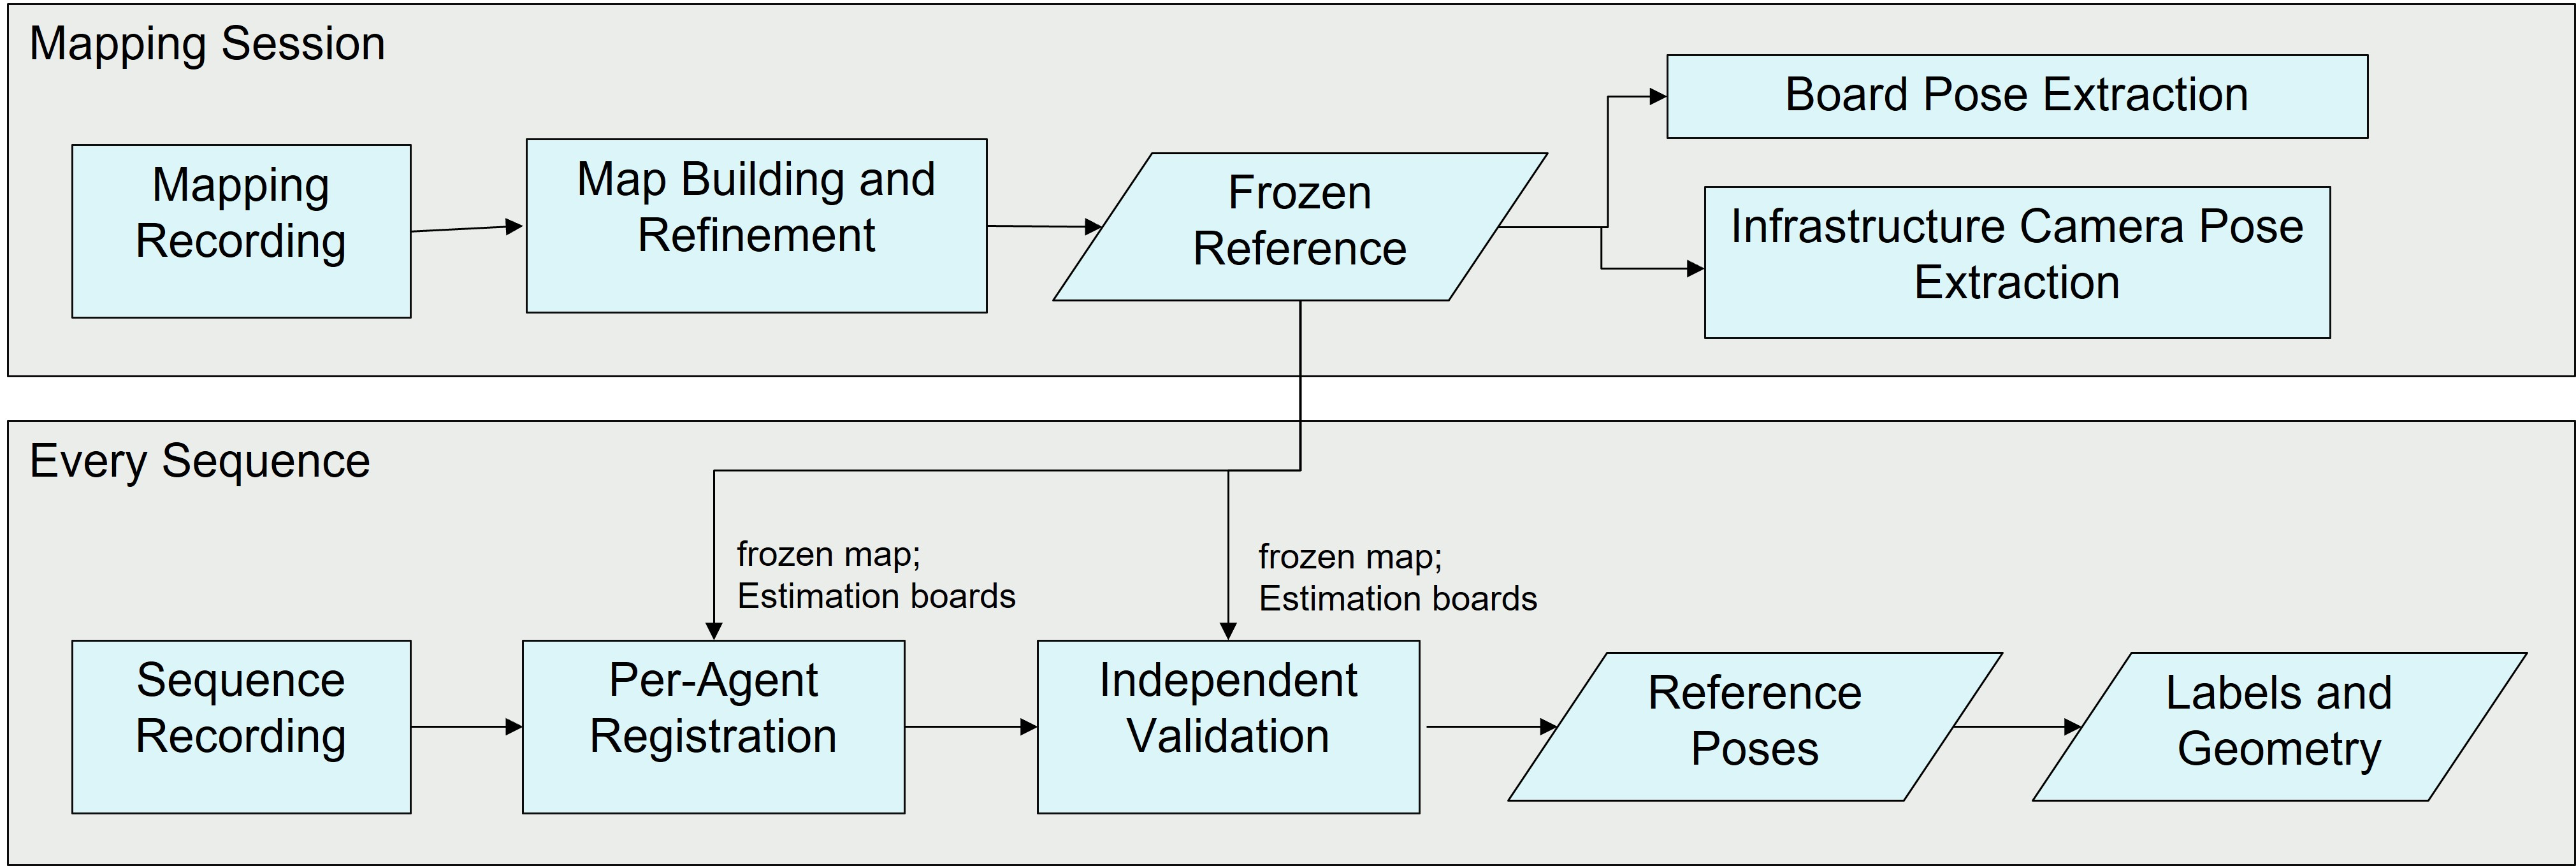
\includegraphics[width=\textwidth]{figs/fig_refpipeline.jpg}
\caption{Reference pipeline. Top: the mapping session, run once per
site, builds and refines the map, poses the boards in it
(Eq.~\eqref{eq:board_chain}), and places the infrastructure cameras
through the boards (Eq.~\eqref{eq:infra_camera_chain}). Bottom: each
sequence is registered into the frozen map, by scan-to-map ICP for the
LiDAR agents and by odometry with ICP and board factors for the RGB-D
agent, and the poses are exported in the site frame.}
\label{fig:refpipeline}
\end{figure*}

\subsection{Reference Map}
\label{sec:map}
% Sec. V-A "Reference Map" for main.tex, with the bundle-adjusted and
% TSDF-fused reference (pass 20261015). To use: replace the body of
% \subsection{Reference Map} in main.tex (from "The reference map is built"
% to "...would not be visible to conventional ICP.") with
% % Sec. V-A "Reference Map" for main.tex, with the bundle-adjusted and
% TSDF-fused reference (pass 20261015). To use: replace the body of
% \subsection{Reference Map} in main.tex (from "The reference map is built"
% to "...would not be visible to conventional ICP.") with
% \input{sections/refmap_main}. Full method and equations:
% supplementary, supp/refmap_method.tex.
The reference map is built in a dedicated mapping session and held fixed
afterwards; no recorded run contributes to it. A LiDAR-inertial SLAM
solution \cite{glim} gives the initial trajectory. It is refined by plane
bundle adjustment \cite{balm,hba}: the poses of \SI{1}{\second} keyframes
are moved jointly so that every planar patch seen from several keyframes is
as thin as possible, the cost of a patch being the smallest eigenvalue of
the scatter of its points, with the SLAM solution's relative motion and
gravity direction kept as soft priors. The scans are then fused into a
truncated signed distance field \cite{curless1996,vdbfusion} with
\SI{2}{\centi\metre} cells and a truncation of \SI{8}{\centi\metre}, three
standard deviations of the spread with which the scans place a wall; the
map is its zero-level surface, and moving objects are removed by
free-space carving \cite{dufomap}. Fusion matters as much as the poses: the
usual union of points keeps every cell a stray point reached, which widened
walls by \SI{4}{\centi\metre} over the scans that built them, whereas the
signed distance averages across a surface. Each stage is measured by the
thickness of the map's planar surfaces (Table~\ref{tab:refmap_stages}):
from the SLAM solution alone to the reference, walls go from
\SI{14.3}{\centi\metre} to \todo{} and floors from \SI{3.6}{\centi\metre}
to \todo{}, and the doubled surfaces left by drift between visits fall
from 2.0\,\% to \todo{}. Against the reference, the SLAM trajectory's error
is a heading error of about $0.6^\circ$ that builds within
\SI{10}{\second} and does not grow further, with an ATE of \todo{}
(Table~\ref{tab:glim_vs_ref}). Bundle adjustment started from two
different trajectories reaches the same poses to \SI{0.7}{\centi\metre}
(median, after alignment) and $0.1^\circ$, so the result is fixed by the
scans and not by the starting point.
. Full method and equations:
% supplementary, supp/refmap_method.tex.
The reference map is built in a dedicated mapping session and held fixed
afterwards; no recorded run contributes to it. A LiDAR-inertial SLAM
solution \cite{glim} gives the initial trajectory. It is refined by plane
bundle adjustment \cite{balm,hba}: the poses of \SI{1}{\second} keyframes
are moved jointly so that every planar patch seen from several keyframes is
as thin as possible, the cost of a patch being the smallest eigenvalue of
the scatter of its points, with the SLAM solution's relative motion and
gravity direction kept as soft priors. The scans are then fused into a
truncated signed distance field \cite{curless1996,vdbfusion} with
\SI{2}{\centi\metre} cells and a truncation of \SI{8}{\centi\metre}, three
standard deviations of the spread with which the scans place a wall; the
map is its zero-level surface, and moving objects are removed by
free-space carving \cite{dufomap}. Fusion matters as much as the poses: the
usual union of points keeps every cell a stray point reached, which widened
walls by \SI{4}{\centi\metre} over the scans that built them, whereas the
signed distance averages across a surface. Each stage is measured by the
thickness of the map's planar surfaces (Table~\ref{tab:refmap_stages}):
from the SLAM solution alone to the reference, walls go from
\SI{14.3}{\centi\metre} to \todo{} and floors from \SI{3.6}{\centi\metre}
to \todo{}, and the doubled surfaces left by drift between visits fall
from 2.0\,\% to \todo{}. Against the reference, the SLAM trajectory's error
is a heading error of about $0.6^\circ$ that builds within
\SI{10}{\second} and does not grow further, with an ATE of \todo{}
(Table~\ref{tab:glim_vs_ref}). Bundle adjustment started from two
different trajectories reaches the same poses to \SI{0.7}{\centi\metre}
(median, after alignment) and $0.1^\circ$, so the result is fixed by the
scans and not by the starting point.


\paragraph{A coloured mesh.} The zero-level surface of the signed
distance field is extracted as a mesh, and its colours come from a 3D
Gaussian splatting model \cite{kerbl2023gaussian} trained on the
mapping session's camera images at their reference poses
\unsure{state how the splats' colours are transferred to the mesh
vertices or faces}. The same map is thus a metric reference for poses
and an appearance reference for rendering: a view rendered from it at a
held-out camera pose can be compared with the image that camera
recorded, \todo{PSNR / SSIM / LPIPS on held-out views}.

The frozen map is the metric backbone of every run. LiDAR agents are
localized by scan-to-map registration. For \texttt{mobile\_2}, depth
registration, visual odometry, and a subset of the board sightings of
Sec.~\ref{sec:fiducials} are combined in one pose-graph optimization
per run, with the selected boards entering as absolute pose factors;
the remaining boards are held out for validation. The LiDAR agents
need no board factors, so for them every board sighting is a
validation measurement. All trajectories therefore share one metric
frame by construction, inter-agent relative poses reduce to two
registration errors against shared local geometry instead of two
accumulated drifts, and since no run contributes to the map, each
agent's agreement with it is an out-of-sample check (reference map and
fiducial network shown in the supplementary material).

\subsection{Fiducial Chain for Agents Without LiDAR}
\label{sec:fiducials}
A sensor-constrained agent cannot enter the map by registration alone:
a cold-start ICP against a building-scale map may converge in a wrong
basin, and between registrations visual odometry accumulates drift,
fastest in feature-poor regions. We therefore deploy a network of
printed ChArUco boards, placed mainly in feature-poor regions where
both visual tracking and depth registration are weakest. The boards
are not surveyed: the pose of each is estimated in the reference frame
from the observations of the mapping session itself, so the network
inherits the metric accuracy of the map. This is sparse anchoring as
in \cite{airmuseum}, with the anchors posed by the map instead of by
survey equipment. During the mapping session the mapping agent stops
at each board to record several views; with the mapping trajectory
\Ttransform{World}{LiDAR} and the extrinsic
\Ttransform{LiDAR}{MobileCamera}, the pose of each board is
\begin{equation}
   \Ttransform{World}{Board} = \Ttransform{World}{LiDAR} \times \Ttransform{LiDAR}{MobileCamera} \times \Ttransform{MobileCamera}{Board} .
   \label{eq:board_chain}
\end{equation}
One board serves as the origin of the world frame, and every mobile
agent starts at a board, so that each run begins at a known pose.
Infrastructure masts are placed in the same frame through a board shown
simultaneously to a mobile and an infrastructure camera:
\begin{equation}
\begin{split}
  \Ttransform{World}{InfraCamera} = {}
    & \Ttransform{World}{LiDAR} \times \Ttransform{LiDAR}{MobileCamera} \times \\
    &  (\Ttransform{Board}{MobileCamera})^{-1} \times \Ttransform{Board}{InfraCamera} .
\end{split}
\label{eq:infra_camera_chain}
\end{equation}
Board sightings thus serve as initialization at the start of a run, as
drift bounds along it, and as validation of every subsequent run.

\subsection{Validation}
\label{sec:gt_val}
Convergence of the refinement establishes self-consistency, not
accuracy: the plane targets are themselves estimated from the map, so
a self-consistent deformation would converge equally well. Accuracy is
therefore established by four checks that did not enter the
estimation (Table~\ref{tab:gt}; error distributions in the
supplementary material).

\paragraph{Surface thickness and a second pass.} Surfaces are measured
by their thickness, the p95--p5 spread of points about planes fitted to
\SI{0.25}{\metre} patches, against the noise of single sweeps, which
carry no pose error (walls \SI{3.0}{\centi\metre}, floors
\SI{1.4}{\centi\metre}). The reference reaches
\SI{7.6}{\centi\metre} on walls and \SI{1.8}{\centi\metre} on floors;
walls, seen at longer range and shallower incidence, stay above the
noise, most in single-visit corridors. A second pass by the other robot
checks the reference across robots and days:
\texttt{mobile\_1}, whose OS1-64 has half the beams of \texttt{mobile\_2}'s OS1-128,
mapped the site three weeks before the reference pass, processed by the
same pipeline with the same settings (board loop closure
\SI{3.2}{\milli\metre}, within its detection noise). Registered rigidly
onto the reference, 96.4\,\% of its surface lies within
\SI{10}{\centi\metre} of the reference's (registration RMS
\SI{3.0}{\centi\metre}), and it covers 86.2\,\% of the reference:
91--92\,\% within \SI{4}{\metre} of the reference path, falling to
46\,\% beyond \SI{12}{\metre}, consistent with its sparser vertical
sampling leaving distant cells below the fusion's three-hit minimum.
The two passes' board-anchored frames differ by \SI{0.49}{\metre} and
$2.95^\circ$ \todo{cause: boards re-mounted between the passes, or a
different anchor board?}, so maps of different passes are compared after
registration.

\paragraph{Control distances.} Laser-rangefinder distances between
landmarks such as opposite walls establish the absolute scale, which
the second pass, sharing the pipeline, cannot: a deformation common to
both passes would shorten or lengthen them alike. Over \todo{$N$}
distances of \todo{a}--\todo{b}\,\si{\metre}, the map agrees with the
rangefinder to about \SI{2}{\centi\metre} RMS \todo{max; relative
error}, so the reference is metric at building scale, not only
self-consistent.

\paragraph{Held-out boards.} When an agent sights a board during a
run, its registered pose and camera extrinsic predict where the board
should appear; the difference from the observed board pose is a
residual that did not enter the registration. Since the boards were
posed from the mapping session, the residual measures how well a run
agrees with the map, not the map's absolute accuracy. On coop2\_0828 (two
agents, one room, \SIrange{146}{152}{\second}, \SIrange{26}{31}{\metre}
of path, three boards, LiDAR held out of every estimate it scores) the
residual is \SI{10.0}{\milli\metre} / 0.88$^\circ$ for
\texttt{mobile\_1} and \SI{54.0}{\milli\metre} / 1.38$^\circ$ for
\texttt{mobile\_2}. The first is fully independent, since the LiDAR
reference consumes no board; its uncertainty is \SI{15}{\milli\metre}.
On coop\_2, whose longer route crosses feature-poor sections, the
RGB-D cart's held-out residual is \SI{3.1}{\centi\metre} median with a
per-pose marginal $\sigma$ of \SI{5.3}{\centi\metre}; without the
map-fix factors the same pose graph reaches \SI{284}{\centi\metre},
which is what the fiducial chain and map registration buy a
sensor-constrained agent. \todo{Report p95 and the board split per
site once all passes are processed.}

\paragraph{Cross-robot consistency.} Where the same surface is observed
by the same robot minutes apart and by different robots on overlapping
routes, the surface agreement tests the full chain of each robot
(registration, extrinsics, time association) at LiDAR accuracy for the
LiDAR pair, and isolates the sensor-constrained mechanism for the
RGB-D cart. \todo{Report.}

\begin{table}[!t]
\centering
\caption{Pseudo Ground Truth Map Quality}
\label{tab:gt}
\begin{tabular}{llc}
\toprule
& Quantity & Value \\
\midrule
\multicolumn{3}{l}{\emph{Surface geometry}} \\
\quad Thickness, seq.\ A & walls / floors & 7.9 / 2.1 cm \\
\quad Thickness, seq.\ B & walls / floors & 9.7 / 2.4 cm \\
\quad Sensor noise floor & walls / floors & 2.9 / 1.25 cm \\
\quad Cross-session      & surface placement, walls & 1.06 cm \\
\quad Cross-session      & relative scale & 0.99998 \\
\quad Control distances  & rangefinder, median & -- \\
\midrule
\multicolumn{3}{l}{\emph{Pose consistency}} \\
\quad Refinement         & final pose correction & 0.15 cm, 0.017$^\circ$ \\
\quad Held-out boards    & LiDAR robot, coop2\_0828 & 10.0 mm, 0.88$^\circ$ \\
\quad Held-out boards    & RGB-D cart, coop2\_0828 & 54.0 mm, 1.38$^\circ$ \\
\quad Held-out boards    & RGB-D cart, coop\_2 (median, $\sigma$) & 3.1 cm, 5.3 cm \\
\quad Repeat-visit       & same robot & -- \\
\quad Cross-robot        & LiDAR vs.\ LiDAR, within 10 cm & 96.4 \% \\
\quad Cross-robot        & coverage of the reference & 86.2 \% \\
\quad Cross-robot        & LiDAR vs.\ RGB-D & -- \\
\bottomrule
\end{tabular}
\end{table}


Each number bounds one error only. A smooth deformation displaces
surfaces without thickening them, so the residual thickness is
per-scan placement scatter; the cross-session comparison bounds the
disagreement between two runs; the control distances bound what both
runs have in common. The reference is centimetre-level and
building-scale from onboard sensing only, and the independent
measurements check the result and never produce it.

\subsection{Scoring Capability}
\label{sec:gt_score}
Because every agent has a pose in the map frame at every scan, an
object labelled once in that frame projects into every agent's frame
through these poses, with the same position, size, and identity across
agents. This is how the testbed scores collaborative perception
without per-frame annotation, and it is why the reference is built to
annotation grade and not only as an evaluation target. The labels
themselves are a release of the dataset \cite{scoop_dataset}.


%=======================================================================
% Sec. Link Instrumentation
\section{Link Instrumentation}
\label{sec:link}
This section answers what the testbed observes of each link, how
often, and within what limits. Fig.~\ref{fig:linktrace} shows one run.
\todo{Extend the figure with RTT and CSI amplitude against time
alongside the agents' positions.}

\subsection{Link State}
Passive metrics are read at \SI{5}{\hertz} from the kernel wireless
interface: RSSI, negotiated bitrate and MCS, transmit retries and
failures, and channel busy ratio. During outages the monitor continues
publishing with \texttt{associated=false}, so coverage gaps appear as
explicit labels and not as missing samples. Active metrics are
obtained with \texttt{iperf3} \cite{iperf3} in \SI{4}{\second} tests,
uplink and downlink separately, in survey or cooperation mode
(Sec.~\ref{sec:decisions}); in cooperation mode the measured goodput
includes the contention a deployed team would face. Latency is
measured as ICMP round-trip time at \SI{100}{\hertz}:
\SI{3.3}{\milli\second} when idle and \SIrange{60}{109}{\milli\second}
under load, the latter caused by queueing and not by path loss.
\todo{The 24 Sep passes give \SIrange{5}{10}{\milli\second} idle and
\SIrange{25}{33}{\milli\second} under iperf load; state both passes
and the load that produced each, or report the range across passes.}

\subsection{Channel State}
\label{sec:csi}
CSI is extracted with Nexmon \cite{nexmon} on a BCM43455c0 in monitor
mode at \SI{80}{\mega\hertz}, which yields one estimate over 242 used
subcarriers per received frame from its VHT-LTF. The extractor,
\texttt{sniffer}, is carried on \texttt{mobile\_1} with a
\SI{2.4}{\giga\hertz} management link kept off the measured band; it
captures the frames of \texttt{mobile\_2} and \texttt{infra\_1}. Only
QoS data frames give full-bandwidth estimates; control frames are
captured for PHY diagnosis but excluded from analysis, since mixing
them changes the effective bandwidth from frame to frame. The achieved
data-frame rates were \SI{141}{\hertz} from \texttt{infra\_1} and
\SI{104}{\hertz} from \texttt{mobile\_2}.

The channel varies over roughly half a wavelength of motion,
$\lambda/2 = \SI{26.1}{\milli\metre}$ at \SI{5745}{\mega\hertz}. If
three estimates per half-wavelength are required to follow these
variations, the achieved rates are sufficient up to a relative speed
of about \SI{1.2}{\metre\per\second}; above that the CSI is too sparse
to resolve them. The rate cannot simply be raised by sending more
packets, since Wi-Fi aggregates many packets into one transmission and
each transmission yields a single channel estimate from its preamble;
disabling aggregation would raise the CSI rate but distort the
throughput being measured. CSI phase is not coherent across devices,
which run on independent oscillators, so each transmitter--receiver
pair is treated as an independent sensing link.

\begin{figure}[t]
\centering
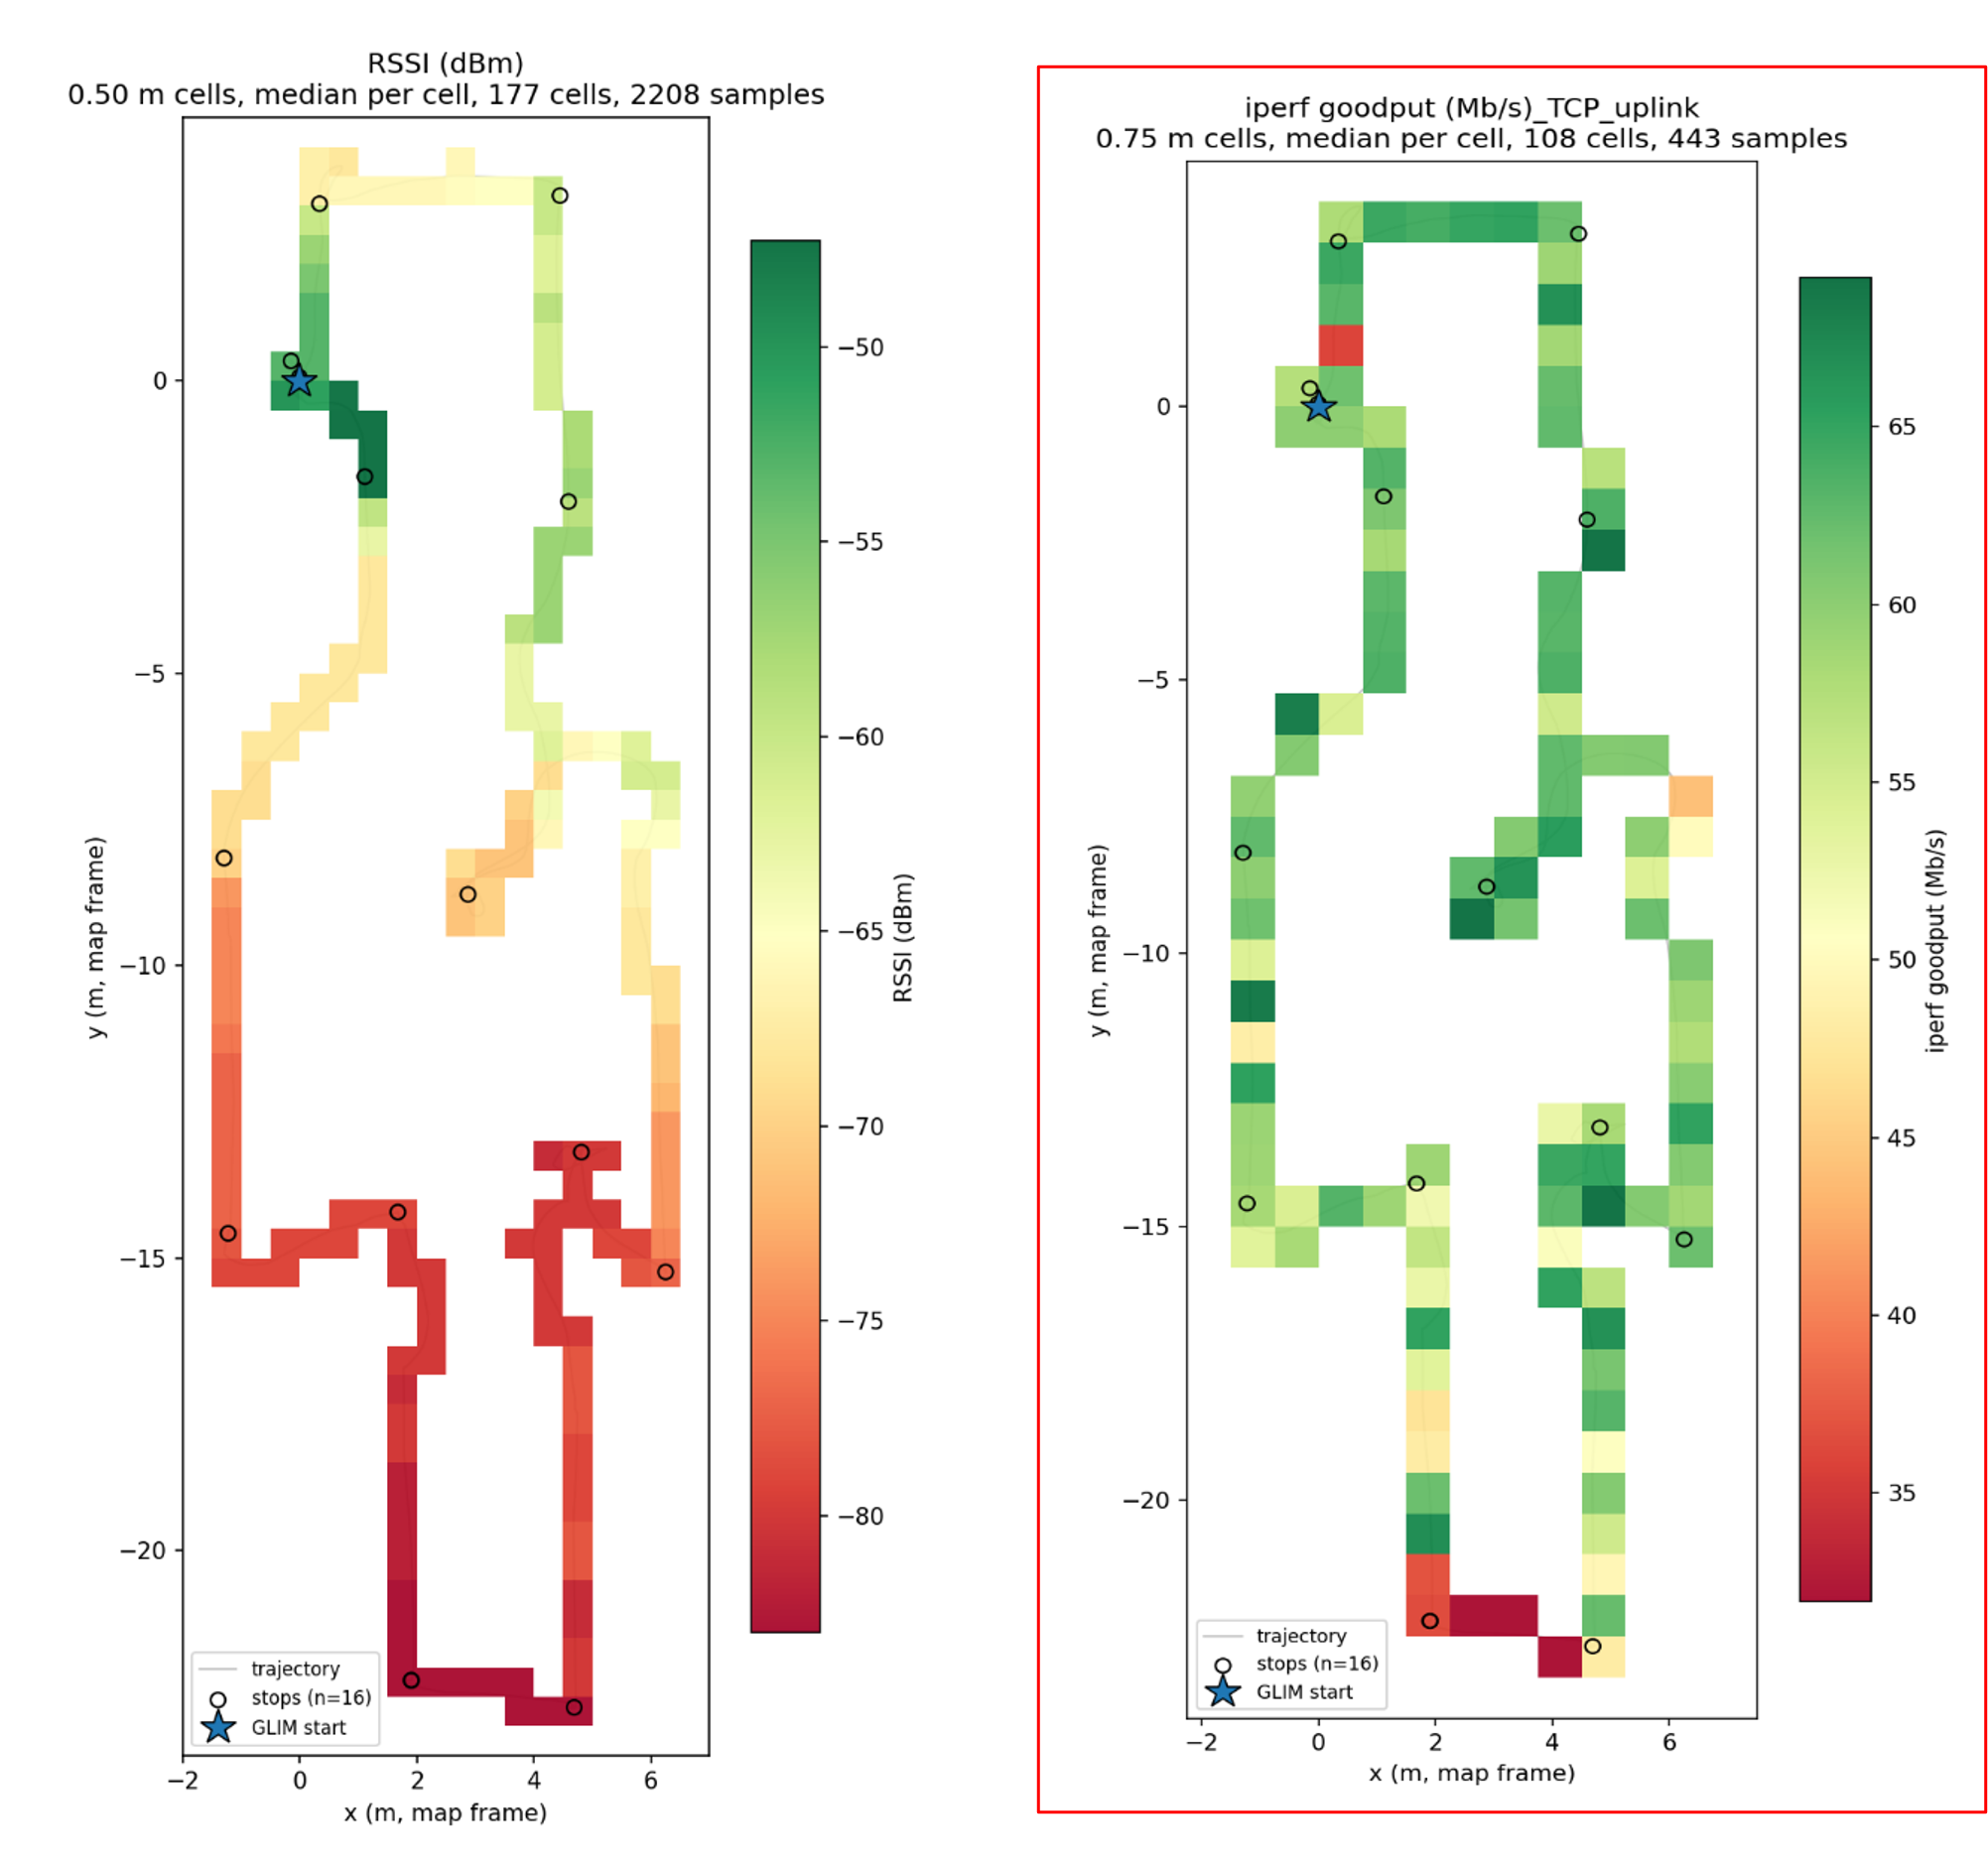
\includegraphics[width=\columnwidth]{figs/fig09_link_trace.png}
\caption{Measured link over one survey sequence at site 1, in the
reference map frame. Left: RSSI, median per \SI{0.5}{\metre} cell
(177 cells, 2208 samples). Right: TCP uplink goodput from
\texttt{iperf3}, median per \SI{0.75}{\metre} cell (108 cells, 443
samples). Circles mark the 16 survey stops, the star the start of the
mapping trajectory.}
\label{fig:linktrace}
\end{figure}



%=======================================================================
% Sec. VII Replay: the recordings as a test bench (about 0.6 page).
% Paragraphs: model; beyond the link (the other recorded conditions);
% interface; positioning.
\section{Replay: The Recordings as a Test Bench}
\label{sec:replay}
This section answers whether any collaborative method can be run on
what the agents sensed and against the link they actually had.

\paragraph{Model.} A message of size $s$ sent at time $t$ over link
$(a,b)$ arrives at
\begin{equation}
  t + d_{ab}(t) + s / G_{ab}(t),
  \label{eq:replay}
\end{equation}
where $d_{ab}(t)$ is the one-way delay and $G_{ab}(t)$ the most recent
goodput measured on that link, and is dropped when the link was down
(\texttt{associated=false}, or a run of lost pings). Because the
measured clock offset is below \SI{1}{\milli\second}, $d_{ab}$ can be
measured directly from stamped probes where they exist, instead of
being assumed to be $\mathrm{RTT}/2$; only a synchronized testbed can
do this. The strict \SI{12}{\milli\second} chrony bound exceeds the
idle one-way delay, so one-way-delay claims rest on the measured
offset, and where probes are absent the module falls back to
$\mathrm{RTT}/2$ and says so. The ideal channel (instant, lossless), the synthetic channels
of prior benchmarks (a fixed bandwidth budget and a fixed or sampled
delay \cite{where2comm,v2xvit,lei2022syncnet,wei2023cobevflow}), and
the logged channel all pass through one module
(Fig.~\ref{fig:replay}), so the channel is the only variable between
runs of a method.

\paragraph{Beyond the link.} The link is one of the conditions the
recordings carry; the others are replayed the same way, each in the
same modes. \emph{Sensors}: a frame that was not recorded is missing in
replay, and the agent is told so (logged); every frame is present
(ideal, where the twin supplies it); or frames drop with each sensor's
measured rate and burst length (fitted). \emph{Pose}: each agent uses
the reference (ideal), its own recorded estimate (logged), or the
reference perturbed with the measured estimate error (fitted). A
method is thus scored with each real-world condition on or off, one at
a time, and a failure is attributed to the condition that caused it
(Sec.~\ref{sec:gym}).

\paragraph{Interface.} Any method that emits (sender, receiver, $t$,
size) plugs in and receives, for each message, an arrival time or a
drop. The implementation extends an OpenCOOD-style wrapper that already
turns latency into staleness and drops collaborators, with a schedule
driven by the trace; a converter places recorded frames in the layout
it reads. \todo{Name the released modules.}

\paragraph{Positioning.} Trace-driven network emulation replays a link
for network software, from trace modulation \cite{noble1997trace}
through netem \cite{hemminger2005netem}, Cellsim
\cite{winstein2013sprout}, Mahimahi \cite{netravali2015mahimahi}, and
Pantheon \cite{yan2018pantheon}; robotics and network co-simulators
couple a robot simulator with a simulated network
\cite{calvofullana2021rosnetsim,sommer2011veins,xu2021opencda};
collaborative-perception benchmarks simulate a link for perception,
and CooperScene \cite{cooperscene} evaluates detectors under one delay
derived from mean measured throughput. SCooP-iT replays the measured
per-message link of each node pair into perception, on the same clock
as the sensors. The fluid model of Eq.~\eqref{eq:replay} is
chosen because the iperf windows give goodput, not per-packet delivery
opportunities as in Mahimahi; E3 measures how much accuracy the simpler
model loses.

\begin{figure}[t]
\centering
\fbox{\parbox[c][4cm][c]{0.95\columnwidth}{\centering
\todo{Fig.: channel-in-the-loop replay. A method emits (sender, receiver,
$t$, size); the module returns an arrival time or a drop from the ideal,
synthetic, or logged channel. Logged: $d_{ab}(t) + s/G_{ab}(t)$, dropped
when the link was down.}}}
\caption{Channel-in-the-loop replay. One module applies the ideal,
synthetic, and logged channels, so the channel is the only variable
between runs of a method.}
\label{fig:replay}
\end{figure}



%=======================================================================
% Sec. VIII Experiments (about 1.6 pages): spec sheet; E1-E4 test the
% instrument; E5 tests what a fitted channel misses.
\section{Experiments}
\label{sec:experiments}
Six tests check the instrument and what it adds (Table~\ref{tab:spec}).
E1 to E4 ask whether the testbed can be trusted; E5 asks whether a
synthetic channel with the same statistics reproduces the logged link; E6
asks whether the twin matches reality and whether what it trains
holds on real data. Each
pass criterion was stated before its test was run. Unless stated
otherwise, link numbers come from the 24 September session at site 1:
\texttt{survey\_1}, in which one agent owns the channel, and
\texttt{coop\_2}, in which both robots move and their active tests
contend. The pose reference is the 15 October mapping pass.

\begin{table*}[!t]
\caption{SCooP-iT Specification Sheet: Every Guarantee, Its Measured Bound, and the Check That Produced It}
\label{tab:spec}
\begin{center}
\renewcommand{\arraystretch}{1.2}
\setlength{\tabcolsep}{4pt}
\scriptsize
\begin{tabular}{@{}p{3.6cm} p{5.2cm} p{5.4cm} p{1.6cm}@{}}
\toprule
\textbf{Guarantee} & \textbf{Bound} & \textbf{Validated by} & \textbf{Experiment} \\
\midrule
Clock agreement between agents & measured offset $\leq$ \SI{0.99}{\milli\second} (\SI{1}{\milli\metre} at \SI{1}{\metre\per\second}); strict chrony bound $\leq$ \SI{12}{\milli\second}; reported RMS offsets \SIrange{10.9}{42.5}{\micro\second} per client & chrony offset logs, every run (coop\_2 so far) & E1 \\
Sniffer clock bias & \todo{to be measured} (worst case \SI{7.8}{\milli\second}) & probe-packet stamps on both ends & E1 \\
Spatial extrinsics & residual per sensor pair, Table~\ref{tab:calib} & held-out reflector and board positions & E1 \\
Agent pose in the site frame & \SI{1.06}{\centi\metre} surface agreement across passes (scale $2\times10^{-5}$); held-out boards \SI{10.0}{\milli\metre} / 0.88$^\circ$ (LiDAR robot), \SI{54.0}{\milli\metre} / 1.38$^\circ$ (RGB-D cart, coop2\_0828) and \SI{3.1}{\centi\metre} median (RGB-D cart, coop\_2); control distances \todo{} & second mapping pass, held-out boards, rangefinder control distances & E1, E2 \\
Link state & \SI{5}{\hertz} passive, \SI{100}{\hertz} RTT, \SI{4}{\second} goodput windows; outages labelled explicitly (3 outages, 12\,\% of frames on coop2\_0828) & monitor publishes through outages; map clearance predicts RSSI ($\rho = 0.60$, \SI{5.4}{\decibel}) & E2, E4 \\
Channel state (CSI) & \SIrange{104}{141}{\hertz}; valid below \SI{1.2}{\metre\per\second} relative speed & $\lambda/2$ sampling argument & --- \\
Contention as a knob & RTT rises several-fold idle to loaded (\SIrange{5}{10}{} to \SIrange{25}{33}{\milli\second}, 24 Sep; \SI{3.3}{} to \SIrange{60}{109}{\milli\second}, earlier pass); in-frame share of \SI{1.5}{\mega\byte} messages 86\,\% alone, \SIrange{59}{68}{\percent} with two robots & survey vs.\ cooperation mode; \todo{repeat across days} & E4, E5 \\
Replay fidelity & \todo{arrival-time error; frame-assignment agreement} & twin run: live payload against replayed trace & E3 \\
\bottomrule
\end{tabular}
\end{center}
\end{table*}


\subsection{E1 Precision: Errors Against Breaking Points}
\emph{Question.} Are the testbed's own errors small next to the errors
at which collaborative fusion breaks? \emph{Pass.} Every term at least
ten times below the breaking point of its kind.

Breaking points are derived for the objects the testbed scores, not
taken from vehicle studies. For a person, a
\SI{0.6}{}$\times$\SI{0.6}{\metre} box in bird's-eye view, a pose error
$d$ along one axis gives an IoU of $0.6(0.6-d)/[0.72-0.6(0.6-d)]$: 0.5 at
$d = \SI{0.20}{\metre}$ and 0.7 at $d = \SI{0.11}{\metre}$. Time errors
are converted to displacement at the measured 95th-percentile speed and
judged against the same points. Each term is plotted on one log axis
against both (Fig.~\ref{fig:headroom}).

\emph{Result.} At IoU 0.5 the measured clock offset (\SI{0.99}{\milli\second},
\SI{1}{\milli\metre} at \SI{1}{\metre\per\second}), the LiDAR robot's
held-out board residual (\SI{10}{\milli\metre}, $20\times$), and the
board detector (\SI{8}{\milli\metre}, $25\times$) pass, and the control
distances (\SI{2}{\centi\metre} RMS, $10\times$) meet the criterion
exactly. Three terms fall
short: the RGB-D cart (\SI{3.1}{\centi\metre} median, $6.5\times$), the
second-pass registration (\SI{3.0}{\centi\metre} RMS, $6.7\times$), and
the strict clock bound (\SI{12}{\milli\second}, $8.3\times$ against one
frame). At IoU 0.7 only the clock, the LiDAR robot, and the detector stay
near $10\times$, and the control distances fall to $5.5\times$; the cart's poses are then only about $3\times$ below the
breaking point, so perception scored from the cart's viewpoint at strict
IoU is limited by the reference. \todo{Fill $v_{95}$, the sniffer bias,
the LiDAR robot on \texttt{coop\_2}, and the radar residuals.}

\begin{figure}[t]
\centering
\fbox{\parbox[c][4.5cm][c]{0.95\columnwidth}{\centering
\todo{Fig.: E1 Headroom. One log axis in metres. Testbed error terms
(clock $\times$ speed, sniffer bias $\times$ speed, extrinsic residuals,
held-out board residual, second-pass agreement) against the fusion
breaking points (\SI{0.2}{\metre} pose error; latency as p95 speed
$\times$ delay against indoor object size \SIrange{0.5}{0.7}{\metre}).}}}
\caption{E1 Headroom: the testbed's own errors against the errors at
which collaborative fusion breaks.}
\label{fig:headroom}
\end{figure}


\subsection{E2 Consistency: The Map Predicts the Radio}
\emph{Question.} Are the poses and the link logs right if neither is
checked by hand? \emph{Pass.} Spearman $\rho > 0.3$ between Fresnel
clearance and the detrended signal, and a clear-minus-obstructed drop
above \SI{5}{\decibel}, on at least one link, with a 95\,\% block-bootstrap
interval excluding zero.

For every window, the first-Fresnel-zone clearance between the two ends
is computed through the map; a path is conventionally clear when
$0.6\,r_1$ of the first Fresnel radius $r_1 = \sqrt{\lambda d_1 d_2/d}$ is
free \cite{itup530}. The distance trend is removed with a fixed
path-loss exponent and an offset from the clear windows; fixing the
exponent keeps the wall loss out of the slope, since along a route
distance and obstruction move together. Neither the map nor the poses
used the signal, so agreement checks both. Intervals use a block
bootstrap over contiguous windows, since neighbouring windows are
correlated. Two confounds are controlled: the cart is pushed by a person
whose body can shadow its antenna, so windows are split by which side of
the cart faces the receiver; and the exponent is varied from 2 to 3.5.

\emph{Result.} On \texttt{coop\_2}, the channel from \texttt{mobile\_2}
to \texttt{mobile\_1}'s position, overheard by the sniffer, gives
$\rho = 0.60$ and a \SI{5.4}{\decibel} drop; the channel from the fixed
\texttt{infra\_1} gives $\rho = 0.23$ and \SI{4.7}{\decibel} and fails,
consistent with a mast whose path to the moving receiver changes less.
A self-test recovers a planted \SI{12}{\decibel} wall loss as
\SI{11.9}{\decibel}. \todo{Bootstrap intervals; exponent sweep; split by
cart side; pooled over \texttt{survey\_1} and \texttt{coop\_2}.}

\begin{figure}[t]
\centering
\fbox{\parbox[c][4cm][c]{0.95\columnwidth}{\centering
\todo{Fig.: E2 Map Meets Radio. Residual signal (dB, distance trend
removed with a fixed path-loss exponent) against Fresnel clearance, per
link and pooled; clear ($\geq 0.6$) vs.\ obstructed ($< 0.6$) windows.}}}
\caption{E2 Map Meets Radio: map-derived Fresnel clearance against the
measured signal it never used.}
\label{fig:clearance}
\end{figure}


\subsection{E3 Replay: Live Arrivals Against Replayed Ones}
\emph{Question.} Does replaying the logged link reproduce the arrivals a
method would see live? \emph{Pass.} At least 90\,\% agreement on the
receiver frame (\SI{100}{\milli\second}) in which each message lands, and
the logged channel closer than the fitted one.

On the \texttt{survey\_1} route, run A records the link as usual, and
run B, back to back, replaces the active tests with a payload node that
sends stamped messages at \SI{10}{\hertz} of \SI{1}{\kilo\byte},
\SI{100}{\kilo\byte}, and \SI{1.5}{\mega\byte} over the transport a
collaborative method uses (ROS~2, best effort), alone and with the other
robot sending; the same pair is repeated in cooperation mode. The
synchronized clocks give each message's one-way delay. B's messages are
replayed through A's trace and through the fitted and published
channels, and the arrival error, frame agreement, and drop agreement are
reported per size and mode (Fig.~\ref{fig:simgap}, left). If a size or
mode fails, the fluid model of Eq.~\eqref{eq:replay} is the limitation
and a per-packet trace \cite{nemfi} is the remedy. \emph{Result.}
\todo{Run the session.}

\subsection{E4 Repeatability: Same Setting, Same Link}
\emph{Question.} Does the same route and mode give the same link on
another day? \emph{Pass.} The day-to-day Wasserstein distance between
the RTT and goodput distributions is below half the distance between
survey and cooperation mode on the same route. \emph{Result.}
\todo{Mode distance from \texttt{survey\_1} and \texttt{coop\_2}; day
distance from the E3 session.}

\subsection{E5 Gap: What a Fitted Channel Misses}
\emph{Question.} Does a synthetic channel with the logged link's
statistics deliver messages as the logged link does? The fitted and
logged channels are compared, and the published channels are shown for
reference; there is no pass criterion, and either outcome is reported.
What the gap costs collaborative SLAM and perception, across methods
and sites, is measured on the SCooP dataset \cite{scoop_dataset}.

\emph{Setup and result.} Messages of \SI{1}{\kilo\byte}, \SI{100}{\kilo\byte},
and \SI{1.5}{\mega\byte} are sent through each channel at \SI{10}{\hertz}.
Under the logged link the predicted share of \SI{1.5}{\mega\byte} messages
that arrive within one frame is 86\,\% with one robot on the channel and
\SIrange{59}{68}{\percent} with two, while the loaded round trip,
\SIrange{25}{33}{\milli\second}, stays well inside the frame. The published
channels deliver 100\,\% by construction: V2X-ViT's constant
\SI{100}{\milli\second} sits on the inclusive frame boundary, and
Where2comm has no delay. These numbers are predictions of
Eq.~\eqref{eq:replay} until E3 validates it, and two robots sending raw
clouds at \SI{10}{\hertz} offer \SI{240}{\mega\bit\per\second}, close to the
measured goodput, so the share is also reported against offered load
divided by goodput, to separate a capacity limit from the link's
structure. \todo{Fitted column; share against normalized load.}

\begin{figure*}[t]
\centering
\fbox{\parbox[c][4.5cm][c]{0.95\textwidth}{\centering
\todo{Left (E3): replayed against live arrival per message, by size and
mode, for the logged and fitted channels. Right (E5a): in-frame share of
1\,KB, 100\,KB, and 1.5\,MB messages under the published, fitted, and
logged channels, survey and cooperation mode, against offered load over
goodput.}}}
\caption{Left, E3: replayed against live message arrivals. Right, E5a:
the logged link against a synthetic channel with the same statistics and
against the published channels of prior benchmarks.}
\label{fig:simgap}
\end{figure*}


\subsection{E6 Twin: The Twin Against Held-Out Passes}
\emph{Question.} Does the twin reproduce held-out real passes?
\emph{Pass.} Synthetic
scans at the recorded poses within \SI{3}{\centi\metre} median of the real
scans; fitted dropout rates and burst lengths within the spread between
real sessions; the place-indexed link predicting the held-out pass's
in-frame share within 10 points and closer than the fitted channel.

\emph{Setup.} The twin drives the recorded paths of a held-out
pass; its scans are registered to the map and compared with the real
scans at the same poses, its camera views are compared with the
recorded images at the same poses, and the dropout and link models fitted on the
build passes are compared with that pass. Whether models trained in
the twin hold on real recordings needs labels and is reported with the
SCooP dataset \cite{scoop_dataset}. \emph{Result.} \todo{Run the twin
on a held-out pass.}



%=======================================================================
% Sec. IX SCooP-iT Gym (about 1.4 pages).
% Paragraphs: the three uses; world built from real data (Table gym_world);
% interface; conditions and augmentation; tasks (Table gym); the
% train-test-deploy protocol; demonstrations; scope.
% Code: ../scoop_gym (link engine, attribution log, CommSchedule-v0, runner);
% world: ../isaac_coop_sim (USD scene from the map, sensors, actors).
\section{SCooP-iT Gym: Train in the Twin, Test on the Recordings, Deploy on the Testbed}
\label{sec:gym}
Recordings answer what happened; they cannot answer what an agent
would have seen had it moved elsewhere. SCooP-iT Gym is a closed-loop
multi-agent environment for that question, and it is tied to the real
testbed at both ends. Its world is built from the recordings, each of
its parts is checked against real runs that did not build it (E3b), a
policy trained in it is tested on the recordings through the replay of
Sec.~\ref{sec:replay}, and the policy is finally deployed on the real
agents (E3c), whose new recordings recalibrate the world. Lingjing
\cite{lingjing} is the nearest environment and supplies the contract we
follow: scenario files, engine-side adjudication, and replayable
episodes with failure attribution. What SCooP-iT Gym changes is the
world and the network: both are measured rather than generated, and
every message is late or lost as it was on the testbed.

\subsection{A World Built from Real Data}
Table~\ref{tab:gym_world} lists the parts of the world, what each is
built from, and how each is checked. The building is the reference map
of Sec.~\ref{sec:gt}, exported to Isaac Sim \cite{isaacsim} as a USD
stage in the map frame with its scanned colours and a collision
surface. The robots are the real platforms: the LiDAR robot as a
differential drive with its measured speed limits, the cart and the
walkers along speed profiles taken from the recordings, the masts
fixed. Each carries the sensors of Table~\ref{tab:sensors} at the
extrinsics of Table~\ref{tab:calib}, with the real LiDAR beam patterns
(64 and 128 beams) and the calibrated camera intrinsics. Localization
is simulated as the true pose plus the error measured between the
agents' estimates and the reference. The link is indexed by place:
per map cell, the round trip and goodput the survey measured there,
scaled by the contention mode measured between survey and cooperation
passes, with outages made more likely where the map's Fresnel clearance
is low, which E2 supports; ray tracing on the same mesh
\cite{hoydis2023sionnart} fills cells the survey did not reach, offset
to agree with the cells it did.

\begin{table}[!t]
\centering
\caption{The Gym's World: What Each Part Is Built From, and How It Is Checked}
\label{tab:gym_world}
\footnotesize
\setlength{\tabcolsep}{3pt}
\begin{tabular}{@{}p{1.4cm} p{3.4cm} p{3.0cm}@{}}
\toprule
Part & Built from & Checked by (E3b) \\
\midrule
Building & reference map (TSDF surface, scan colours) & synthetic vs.\ real scans at the same poses \\
Sensors & beam patterns, intrinsics, extrinsics; noise and dropouts fitted per sensor & held-out session statistics \\
Motion & platform limits; recorded speed profiles & recorded commands reproduce recorded paths \\
Localization & measured estimate-vs.-reference error & held-out error statistics \\
Link & survey per cell, contention mode, clearance; ray tracing where unsurveyed & prediction along a held-out pass \\
Objects & labels (classes, counts per room); object bank & detector with and without, tested on real data \\
\bottomrule
\end{tabular}
\end{table}

\subsection{Interface}
Each task is an Isaac Lab \cite{orbit} multi-agent environment behind
the Gymnasium and PettingZoo interfaces \cite{gymnasium,pettingzoo}, so
it runs many instances in parallel for training. At every step the
simulator renders each agent's sensors and moves the agents; a
simulator-independent layer, the same code that drives the replay,
decides which messages arrive, applies the conditions, computes the
reward from exact ground truth, and writes the attribution log. An
agent observes its own sensor frames, its own pose estimate, the
messages that arrived, and its own link monitor (last round trip and
goodput); it acts by moving (velocity or waypoint), by communicating
(what to send, and to whom), and, where the task asks, by choosing how
to fuse. Each failure is logged with one cause: a sensor dropout, a
pose error, an occlusion no agent overcame, or the link, itself split
into outage, queue, transmission, and latency.

\subsection{Conditions and Augmentation}
Each real-world condition is a setting in the scenario file with the
four modes of the replay: \emph{ideal}, \emph{logged}, \emph{fitted}
from the measured statistics, and, for training only,
\emph{augmented}. This covers the link, sensor availability and noise,
pose error, and objects. The recordings have few objects and some
sensor dropouts; the Gym addresses both without touching the
evaluation. Objects are placed in the stage at positions sampled from
the map's free space, at class counts taken from the labels, with rare
configurations added on purpose (a person visible to a mast but
occluded from every robot); every sensor of every agent sees them at
once, each with its own occlusion, and each carries an exact box and a
semantic class. Dropouts are drawn from each sensor's measured rate
and burst length. One rule keeps this honest: augmented and twin data
may enter training, and only real recordings enter evaluation.

\subsection{Tasks}
Table~\ref{tab:gym} lists the environments. Closed-loop tasks run in the
twin, where acting changes what is perceived and how the link behaves;
replay tasks run on the recordings, where the motion is the recorded
one and the agents choose what to sense, send, and fuse.

\begin{table}[!t]
\centering
\caption{SCooP-iT Gym Environments}
\label{tab:gym}
\footnotesize
\setlength{\tabcolsep}{3pt}
\begin{tabular}{@{}l l p{3.4cm}@{}}
\toprule
Environment & Mode & Agents decide; reward \\
\midrule
\texttt{OcclusionHandoff} & twin & mast warns robot of an occluded person, robot slows; no conflict, little delay \\
\texttt{ActiveCoopDetect} & twin & where a helper moves to see what the ego cannot; detection gain \\
\texttt{CoopSearch} & twin & team search for a labelled object; time to find \\
\texttt{ConnectedCoverage} & twin & motion and sync; area and data, minus lost links \\
\texttt{RelayPlacement} & twin & where to park as relay; time connected \\
\midrule
\texttt{CoopDetect} & replay & what to share and how to fuse; detection gain over ego \\
\texttt{HelperSelect} & replay & which helper to ask; detection gain \\
\texttt{CommSchedule} & replay & message kind per frame; value in deadline minus airtime \\
\bottomrule
\end{tabular}
\end{table}

\subsection{Train, Test, Deploy}
A method is trained in the twin, with any conditions and augmentation;
tested on the recordings, where the replay covers its perception and
communication with every condition logged; and deployed on the
testbed, where the outcome is compared with the Gym's prediction
(E3c). The deployment's recordings return to the first step and refit
the conditions and the link, so the Gym is recalibrated by every use of
the testbed.

\subsection{Demonstrations}
\texttt{CommSchedule} runs today on the recordings: per LiDAR frame, a
sender chooses nothing, boxes (\SI{1}{\kilo\byte}), features
(\SI{100}{\kilo\byte}), or the raw cloud (\SI{1.5}{\mega\byte}). Under
the ideal and synthetic channels the best policy always sends the raw
cloud; under the logged link a rule that sends it only when the
monitored goodput would land it within the frame \todo{raises the
in-frame share from X to Y\,\% on \texttt{coop\_2}}.
\texttt{OcclusionHandoff} carries the full protocol: \todo{trained in
the twin; tested on the \texttt{coop\_2} recordings; deployed on the
testbed (E3c)}.

\paragraph{Scope} The twin is geometric: it renders the surfaces the
map has with the appearance the scans gave them, so camera tasks
inherit an appearance gap that the objects' materials and lighting are
randomized to reduce and that E3b measures. The link indexed by place
is a model, validated only as far as E3b's held-out pass reaches.


%=======================================================================
% Sec. X Lessons from the real world, and limitations (about 0.5 page).
% One paragraph per lesson, each with its number; then the limits.
\section{Lessons from the Real World, and Limitations}
\label{sec:lessons}
Each lesson below is a condition the real testbed imposed that a
simulator would not have, and each is now a condition the Gym
reproduces.

\paragraph{CSI constraints shape the network.} Commodity CSI extraction
imposed a single spatial stream, 802.11ac rather than ax, and
\SI{80}{\mega\hertz} on every transmitter, and aggregation caps the
CSI rate at roughly \SIrange{100}{140}{\hertz} under load, sufficient
only below about \SI{1.2}{\metre\per\second}. These are constraints of
the measurement, not of the robots, and must accompany any throughput
number recorded on the platform; raising the CSI rate by disabling
aggregation would distort the throughput being measured.

\paragraph{NTP asymmetry on the sniffer's management link.} Reaching
the CSI host over a second wireless hop introduced the only clock bias
the protocol cannot observe. Probe packets stamped on both ends
measure it; a wired connection to \texttt{mobile\_1} removes it.
\todo{Confirm once the Ethernet change is made.}

\paragraph{Cold-start ICP falls into wrong basins at building scale.}
Hence boards go in feature-poor regions and every run starts at a
board.

\paragraph{Check the SLAM solution's clock before refining it.} The
SLAM poses were stamped \SI{46}{\milli\second} early; uncorrected,
this alone made the heading wrong by about $1^\circ$ while turning and
walls \SI{18.8}{\centi\metre} thick over the run instead of
\SI{12.0}{\centi\metre}. Fusion is the second
term: a union of points kept walls \SI{5}{\centi\metre} thicker than
the signed-distance fusion of the same scans.

\paragraph{Sensors fall short of their nominal rate.} Recorded at full
resolution with lossless compression, the stereo camera wrote about one
frame per second instead of 15 in one cooperative session, a shortfall
the robot's disk imposed and no driver reported. Rates are therefore
logged per stream, the release flags frames that are missing, and the
Gym's dropout condition is fitted to them.

\paragraph{Limits.} One band and one protocol; one access point per
site; one CSI receiver; the self-built map rests on the control
distances for absolute scale, since the two passes share a sensor and
a pipeline; endpoint clearances hide obstacles within
\SI{0.7}{\metre} of a radio. \todo{Add scale: three sites, sessions,
hours, once final.} On real data the loop is open: the nodes do not act
on what they receive, and a replayed trace cannot react to the load a
method offers. It closes only in the twin, whose sensors are geometric,
without reflectance, dropout, or motion distortion, and whose link, once
agents leave the recorded paths, is a model indexed by place rather than
a trace. The step from received message to action, which closes the
loop of networked embodied intelligence \cite{zhang2026mean}, is
therefore learned in simulation and checked on the testbed only through
deployment (E3c).


%=======================================================================
% Sec. XI Conclusion (about 0.2 page): what it gives, what it showed, what is next.
\section{Conclusion}
\label{sec:conclusion}
SCooP-iT captures a real heterogeneous indoor team, sensing and
communication alike, on one clock, with measured offsets below
\SI{1}{\milli\second}, and in one metric frame, placed to
\SI{10}{\milli\metre} against held-out boards without motion capture or
GNSS. The capture serves three uses, each checked against reality: the
recordings as a test bench into which any collaborative method is
replayed against the link the agents had \todo{validated to within one
receiver frame}; SCooP-iT Gym, a closed-loop environment whose world,
sensors, link, and conditions are built from the recordings; and the
testbed itself, on which a policy trained in the Gym is deployed and
its outcome compared with the Gym's prediction. The real world showed
what simulation hides: under contention the shared network moves raw
clouds past one LiDAR frame while its own latency looks healthy, which
no synthetic channel of prior benchmarks reproduces. Next steps are more
agents and sites, other radios, multi-antenna CSI, a wired CSI host, and
Gym tasks in which agents act on the real testbed in closed loop. The
sequences recorded on SCooP-iT, their labels, and their benchmark are
released as the SCooP dataset \cite{scoop_dataset}.


\section*{Acknowledgment}
\todo{Add acknowledgments in this section.}

\bibliographystyle{IEEEtran}
\bibliography{references}

% Supporting material is in supplementary.tex (compiled separately):
% full sensor table, topics, clock statistics per client, reference map
% method, GT error distributions, data flow, sensor intrinsics.

\end{document}
